%\documentclass[a4paper, 12pt, listof=list, bibliography=totoc, pointlessnumbers, oneside]{scrreprt}
\documentclass[a4paper, 12pt, listof=totoc, bibliography=totoc]{scrreprt}
%\usepackage[top=2cm, bottom=2cm, left=3.5cm, right=2cm]{geometry}
\usepackage[top=2.5cm, bottom=2.5cm, left=2.5cm, right=2.5cm]{geometry}

\usepackage[utf8x]{inputenc}	%Deutsche Umlaute
\usepackage[ngerman]{babel} 	%Deutsches \chapter, \tableofcontents etc.
\usepackage[T1]{fontenc}		%Schriftsatzerweiter
\usepackage{scrpage2}			%Kopf- und Fußzeile
\usepackage{blindtext}			%Textdokument mit Fließtext erzeugen
\usepackage{todonotes}			%Noch zu erledigen
\usepackage{listings}			%Codebeispiele
\usepackage{setspace}			%Zeilenabstand
%\usepackage[square]{natbib}
\usepackage{float}				%Bilder ach Text
\usepackage{chngcntr}			%Abbildung durchgehen, nicht pro Kapitel nummerieren
\usepackage{tabularx}			%Tabellenbreite begrenzen auf Textbreite
\usepackage{seqsplit}			%Lange Wörter brechen
%\usepackage[withpage, printonlyused]{acronym}			%Abkürzungsverzeichnis
\usepackage{acro}				%Acronyme
\usepackage{enumitem}			%Kompakte Listen

\usepackage{lmodern}			%Sonderzeichen im PDF
\usepackage[]{hyperref}			
\hypersetup{colorlinks=true,allcolors=blue}
%\hypersetup{colorlinks=true,allcolors=black}
\usepackage{hypcap}
\usepackage[parfill]{parskip}
\usepackage{longtable}
\usepackage{hhline}
\usepackage{slashbox}
\usepackage{url}
\usepackage{filecontents}
\usepackage{courier}

\usepackage{svg}
\usepackage{amsmath}
\usepackage{enumitem}
%\usepackage{titlesec}
%\usepackage{hyperref}
%\usepackage{fancybox, graphicx}
%\usepackage{arydshln}

%\usepackage{dirtytalk}
%\usepackage[table]{xcolor}
%\usepackage{graphicx}

\usepackage{pifont}				%Extra Ascii Icons
\usepackage{makeidx}			%Stichwortverzeichnis
%fehlt noch 
\newcommand{\missing}[1]{\todo[color=red!40, inline]{#1}}
%fehlt noch alles
\newcommand{\missingall}{\todo[color=red!40, inline]{Fehlt komplett...}}
%fehlt noch etwas
\newcommand{\missingtext}{\todo[color=red!40, inline]{Mehr Text}}
%fehlt Quelle
\newcommand{\missingcite}{\todo[color=red!40, inline]{Quelle}}

%Anführungszeichen
\newcommand{\quotes}[1]{\glqq #1\grqq}
%Anführungszeichen
\newcommand{\fr}[1]{\frqq #1\flqq}
%Prozentsymbol
\newcommand{\percent}{\%}

%Linie referenzieren
\newcommand{\lstnumberautorefname}{Linie}

%url
\newcommand{\pseudourl}[1]{\textit{\seqsplit{#1}}}

%Datei- oder Order
\newcommand{\filefolder}[1]{\texttt{\seqsplit{#1}}}

%Inline Code
\newcommand{\inlinecode}[1]{\texttt{\seqsplit{#1}}}

%Hostname für Server A und Server B und Proxy Server
\newcommand{\hostnameA}{\pseudourl{aem.example.com}}
\newcommand{\hostnameB}{\pseudourl{www.example.com:3000}}
\newcommand{\hostnameP}{\pseudourl{cdn.example.com}}

%Url Präfix für Server A und Server B und Proxy Server
\newcommand{\serverA}[1][]{\pseudourl{http://\hostnameA/#1}~}
\newcommand{\serverAN}[1][]{\pseudourl{http://\hostnameA/#1}}
\newcommand{\serverB}[1][]{\pseudourl{http://\hostnameB/spa/#1}~}
\newcommand{\serverBN}[1][]{\pseudourl{http://\hostnameB/spa/#1}}
\newcommand{\serverP}[1][]{\pseudourl{http://\hostnameP/#1}~}
\newcommand{\serverPN}[1][]{\pseudourl{http://\hostnameP/#1}}

%Unvollendete Kapitel hervorheben
\newcommand{\chaptertbd}[1]{\chapter{\textcolor{red}{#1}}}
\newcommand{\sectiontbd}[1]{\section{\textcolor{red}{#1}}}
\newcommand{\subsectiontbd}[1]{\subsection{\textcolor{red}{#1}}}
\newcommand{\subsubsectiontbd}[1]{\subsubsection{\textcolor{red}{#1}}}
\newcommand{\paragraphtbd}[1]{\paragraph{\textcolor{red}{#1}}}
\newcommand{\subparagraphtbd}[1]{\subparagraph{\textcolor{red}{#1}}}

%Tabellenköpfe hervorheben
\newcommand{\thead}[1]{\textbf{#1}}

%Name für AEM+WS Kombonente
\newcommand{\ajc}{\ac{ajc}~}





\pagestyle{scrheadings}
\automark[chapter]{chapter}
\renewcommand{\chapterpagestyle}{scrheadings}
\renewcommand{\indexpagestyle}{scrheadings}

\setlength{\footskip}{1cm}

\setheadsepline{0.5pt}

\ihead{\headmark}
\chead{}
\ohead{\thepage}

\ifoot{\thesubject}
\cfoot{Zwischenabgabe vom \today}
\cfoot{}
\ofoot{\theauthor}
\title{Studie zur Integration von dynamischen Inhalten in CMS-Systeme mit Hilfe von Webframeworks}
\author{Julian Kandler}
\date{--.--.2017}
\subject{Masterarbeit}
%'Codeabschnitt' anstelle von 'Listening'
\renewcommand{\lstlistingname}{Codebeispiel}
%'Codeabschnitverzeichnis' anstelle von 'Listenings'
\renewcommand{\lstlistlistingname}{Codebeispielverzeichnis}


\definecolor{lightgray}{rgb}{0.95, 0.95, 0.95}
\definecolor{darkgray}{rgb}{0.4, 0.4, 0.4}
%\definecolor{purple}{rgb}{0.65, 0.12, 0.82}
\definecolor{editorGray}{rgb}{0.95, 0.95, 0.95}
\definecolor{editorOcher}{rgb}{0.8, 0.2, 0} % #FF7F00 -> rgb(239, 169, 0)
\definecolor{editorGreen}{rgb}{0, 0.5, 0} % #007C00 -> rgb(0, 124, 0)
\definecolor{orange}{rgb}{1,0.45,0.13}		
\definecolor{olive}{rgb}{0.17,0.59,0.20}
\definecolor{brown}{rgb}{0.69,0.31,0.31}
\definecolor{purple}{rgb}{0.38,0.18,0.81}
\definecolor{lightblue}{rgb}{0.1,0.57,0.7}
\definecolor{lightred}{rgb}{1,0.4,0.5}

%Definition der Codeabschnitte
%\lstset{numbers=left, frame=single, captionpos=b}
\lstset{
	backgroundcolor = \color{lightgray},
	basicstyle=\ttfamily\scriptsize,
	numbers=left,
	captionpos=b,
    frame=single,
    breaklines=true,
    postbreak=\raisebox{0ex}[0ex][0ex]{\ensuremath{\color{red}\hookrightarrow\space}}
}






% CSS
\lstdefinelanguage{CSS}{
  keywords={color,background-image:,margin,padding,font,weight,display,position,top,left,right,bottom,list,style,border,size,white,space,min,width, transition:, transform:, transition-property, transition-duration, transition-timing-function},	
  sensitive=true,
  morecomment=[l]{//},
  morecomment=[s]{/*}{*/},
  morestring=[b]',
  morestring=[b]",
  alsoletter={:},
  alsodigit={-}
}

% JavaScript
\lstdefinelanguage{JavaScript}{
  morekeywords={typeof, new, true, false, catch, function, return, null, catch, switch, var, if, in, while, do, else, case, break},
  morecomment=[s]{/*}{*/},
  morecomment=[l]//,
  morestring=[b]",
  morestring=[b]'
}

\lstdefinelanguage{HTML5}{
  language=html,
  sensitive=true,	
  alsoletter={<>=-},	
  morecomment=[s]{<!-}{-->},
  tag=[s],
  otherkeywords={
  % General
  >,
  % Standard tags
	<!DOCTYPE,
  </html, <html, <head, <title, </title, <style, </style, <link, </head, <meta, />,
	% body
	</body, <body,
	% Divs
	</div, <div, </div>, 
	% Paragraphs
	</p, <p, </p>,
	% scripts
	</script, <script,
  %More tags...
  <canvas, /canvas>, <svg, <rect, <animateTransform, </rect>, </svg>, <video, <source, <iframe, </iframe>, </video>, <image, </image>, <header, </header, <article, </article,
  <h1, </h1, <img, <ul, </ul, <li, </li, <form, </form, <input, <link,
  %HTL
  <sly, </sly,
  %Angular
  <Nav, </Nav, <Profile, </Profile
  },
  ndkeywords={
  % General
  =,
  % HTML attributes
  charset=, src=, id=, width=, height=, style=, type=, rel=, href=, alt=, class=, placeholder=, color=,
  % SVG attributes
  fill=, attributeName=, begin=, dur=, from=, to=, poster=, controls=, x=, y=, repeatCount=, xlink:href=,
  % properties
  margin:, padding:, background-image:, border:, top:, left:, position:, width:, height:, margin-top:, margin-bottom:, font-size:, line-height:,
	% CSS3 properties
  transform:, -moz-transform:, -webkit-transform:,
  animation:, -webkit-animation:,
  transition:,  transition-duration:, transition-property:, transition-timing-function:,
  %HTL
  data-sly-list.child=, data-sly-use.clientlib=, data-sly-call=, data-sly-unwrap,
  %Angular
  ng-app, ng-app=, ng-view, ng-model
  }
}

\lstdefinestyle{htmlcssjs} {%
  % General design
%  backgroundcolor=\color{editorGray},
  basicstyle={\footnotesize\ttfamily},   
  frame=b,
  % line-numbers
  xleftmargin={0.75cm},
  numbers=left,
  stepnumber=1,
  firstnumber=1,
  numberfirstline=true,	
  % Code design
  identifierstyle=\color{black},
  keywordstyle=\color{blue}\bfseries,
  ndkeywordstyle=\color{editorGreen}\bfseries,
  stringstyle=\color{editorOcher}\ttfamily,
  commentstyle=\color{brown}\ttfamily,
  % Code
  language=HTML5,
  alsolanguage=JavaScript,
  alsodigit={.:;},	
  tabsize=2,
  showtabs=false,
  showspaces=false,
  showstringspaces=false,
  extendedchars=true,
  breaklines=true,
  % German umlauts
  literate=%
  {Ö}{{\"O}}1
  {Ä}{{\"A}}1
  {Ü}{{\"U}}1
  {ß}{{\ss}}1
  {ü}{{\"u}}1
  {ä}{{\"a}}1
  {ö}{{\"o}}1
}




\lstdefinestyle{xml}
{
  % General design
%  backgroundcolor=\color{editorGray},
basicstyle={\footnotesize\ttfamily},   
frame=b,
% line-numbers
xleftmargin={0.75cm},
numbers=left,
stepnumber=1,
firstnumber=1,
numberfirstline=true,	
% Code design
identifierstyle=\color{black},
keywordstyle=\color{blue}\bfseries,
ndkeywordstyle=\color{editorGreen}\bfseries,
stringstyle=\color{editorOcher}\ttfamily,
commentstyle=\color{brown}\ttfamily,
tabsize=2,
showtabs=false,
showspaces=false,
showstringspaces=false,
extendedchars=true,
breaklines=true,
morestring=[s]{"}{"},
morecomment=[s]{?}{?},
morecomment=[s]{!--}{--},
commentstyle=\color{brown},
moredelim=[s][\color{black}]{>}{<},
moredelim=[s][\color{red}]{\ }{=},
stringstyle=\color{red},
identifierstyle=\color{blue},
% German umlauts
literate=%
{Ö}{{\"O}}1
{Ä}{{\"A}}1
{Ü}{{\"U}}1
{ß}{{\ss}}1
{ü}{{\"u}}1
{ä}{{\"a}}1
{ö}{{\"o}}1
}



\lstdefinestyle{jcr}
{
  % General design
%  backgroundcolor=\color{editorGray},
basicstyle={\footnotesize\ttfamily},   
frame=b,
% line-numbers
xleftmargin={0.75cm},
numbers=left,
stepnumber=1,
firstnumber=1,
numberfirstline=true,
%morecomment=[l]{\#},
%morestring=[b]-,	
% Code design
identifierstyle=\color{black},
keywordstyle=\color{blue}\bfseries,
ndkeywordstyle=\color{editorGreen}\bfseries,
stringstyle=\color{editorGreen}\ttfamily,
commentstyle=\color{brown}\ttfamily,
tabsize=2,
showtabs=false,
showspaces=false,
showstringspaces=false,
extendedchars=true,
breaklines=true,
% German umlauts
literate=%
{Ö}{{\"O}}1
{Ä}{{\"A}}1
{Ü}{{\"U}}1
{ß}{{\ss}}1
{ü}{{\"u}}1
{ä}{{\"a}}1
{ö}{{\"o}}1
}

\emergencystretch=1em

\definecolor{tableheader}{RGB}{240,240,250}
%\bibliographystyle{natdin}
\bibliographystyle{alphadin}

%1,3 facher Zeilenabstand
\setstretch{1.3}

%Table of Content Tiefe
\setcounter{tocdepth}{5}
\setcounter{secnumdepth}{5}

%Durchgehend nummerieren
\counterwithout{figure}{chapter}
\counterwithout{table}{chapter}
\lstset{ numberbychapter=false}

\makeatletter
\let\thetitle\@title
\let\theauthor\@author
\let\thesubject\@subject

%Inhaltsverzeichnis in das Inhaltsverzeichnisq
\setuptoc{toc}{totoc}

%Kapitel nicht einrücken

\renewcommand\paragraph{\@startsection{paragraph}{4}{\z@}%
	{-3.25ex \@plus -1ex \@minus -0.2ex}%
	{0.01pt}%
	{\raggedsection\normalfont\sectfont\nobreak\size@paragraph}%
}


\usepackage{soul}
\definecolor{hl-color}{RGB}{240,240,240}
\sethlcolor{hl-color}
\setsvg{svgpath = src/svg/}

\lstset{literate=%
	{Ö}{{\"O}}1
	{Ä}{{\"A}}1
	{Ü}{{\"U}}1
	{ß}{{\ss}}1
	{ü}{{\"u}}1
	{ä}{{\"a}}1
	{ö}{{\"o}}1
	{~}{{\textasciitilde}}1
}

\graphicspath{{./src/img/}}
\renewcommand{\lstnumberautorefname}{Zeile}

%Abstände in Verzeichniseinträgen entfernen
%\renewcommand*{\addvspace}[1]{}

\DeclareAcronym{cms}{
short = CMS,
long = Content Management System,
foreign = Inhaltsverwaltungssysteme
}
\DeclareAcronym{aem}{
short = AEM,
long = Adobe Experience Manager
}
\DeclareAcronym{seo}{
short = SEO,
long = Search Engine Optimization,
foreign = Suchmaschinenoptimierung
}
\DeclareAcronym{html}{
short = HTML,
long = HyperText Markup Language,
foreign = Hypertext-Auszeichnungssprache
}
\DeclareAcronym{css}{
short = CSS,
long = Cascading Style Sheets,
foreign = gestufte Gestaltungsbögen
}
\DeclareAcronym{dom}{
short = DOM,
long = Document Object Model,
foreign = Dokument Objekt Model
}
\DeclareAcronym{ajax}{
short = Ajax,
long = Asynchronous JavaScript and XML,
foreign = Asynchrones JavaScript und XML
}
\DeclareAcronym{spa}{
short = SPA,
long = Single Page Application,
foreign = Einzelseiten-Webanwendungen
}
\DeclareAcronym{w3c}{
	short = W3C,
	long = World Wide Web Consortium,
}
\DeclareAcronym{xml}{
	short = XML,
	long = Extensible Markup Language,
	foreign = erweiterbare Auszeichnungssprache
}
\DeclareAcronym{json}{
	short = JSON,
	long = JavaScript Object Notation,
}
\DeclareAcronym{mvc}{
	short = MVC,
	long = Model View Controller,
	foreign = Modell-Präsentation-Steuerung
}
\DeclareAcronym{mvvm}{
	short = MVVM,
	long = Model View ViewModel,
	foreign = Modell-Präsentation Präsentationsmodell
}
\DeclareAcronym{amc}{
	short = AMC,
	long = Adobe Marketing Cloud,
}
\DeclareAcronym{jcr}{
	short = JCR,
	long = Content Respository for Java Technologie,
}
\DeclareAcronym{crx}{
	short = CRX,
	long = Content Repository Extreme,
}
\DeclareAcronym{api}{
	short = API,
	long = Application Programming Interface,
	foreign = Programmierschnittstelle,
}
\DeclareAcronym{iso}{
	short = ISO,
	long = International Organization for Standardization,
}
\DeclareAcronym{di}{
	short = DI,
	long = Dependency Injection,
}
\DeclareAcronym{ioc}{
	short = IoC,
	long = Inversion of Control,
}
\DeclareAcronym{htl}{
	short = HTL,
	long = HTML Template Language,
}
\DeclareAcronym{jsp}{
	short = JSP,
	long = JavaServer Pages,
}
\DeclareAcronym{jre}{
	short = JRE,
	long = Java Runtime Environment,
}

\DeclareAcronym{jsx}{
	short = JSX,
	long = JavaScript XML,
}
\DeclareAcronym{jar}{
	short = JAR,
	long = Java Archive,
}
\DeclareAcronym{npm}{
	short = npm,
	long = Node Package Manager,
}

\DeclareAcronym{amd}{
	short = AMD,
	long = Asynchronous Module Definiton,
}
\DeclareAcronym{mpa}{
	short = MPA,
	long = Multi-Page-Application,
}

\DeclareAcronym{webdav}{
	short = WebDAV,
	long = Web-based Distributed Authoring and Versioning,
}
\DeclareAcronym{rest}{
	short = REST,
	long = Representational State Transfer,
}

\DeclareAcronym{url}{
	short = URL,
	long = Uniform Resource Locator,
}

\DeclareAcronym{http}{
	short = HTTP,
	long = Hypertext Transfer Protocol,
	foreign = Hypertext-Übertragungsprotokoll
}

\DeclareAcronym{aot}{
	short = AoT,
	long = Ahead-of-Time,
	foreign = Vorzeitig,
}

\DeclareAcronym{jit}{
	short = JiT,
	long = Just-in-Time,
	foreign = Rechtzeitig,
}

\DeclareAcronym{xhr}{
	short = XHR,
	long = XMLHttpRequest,
}

\DeclareAcronym{cors}{
	short = CORS,
	long = Cross-Origin Resource Sharing,
}

\DeclareAcronym{sop}{
	short = SOP,
	long = Same-Origin-Policy,
}

\DeclareAcronym{sce}{
	short = SCE,
	long = Strong Contextual Escaping,
}

\DeclareAcronym{ajc}{
	short = AJC,
	long = AEM and JavaScript Component,
	foreign = AEM und JavaScript Komponente,	
}


\makeatletter
\renewcommand\subparagraph{\@startsection{subparagraph}{4}{\z@}%
	{-3.25ex \@plus -1ex \@minus -0.2ex}%
	{0.01pt}%
	{\raggedsection\normalfont\sectfont\nobreak\size@subparagraph}%
}
\makeatother



%Zum Testen alle Bilder ausblenden
%\renewcommand*\includegraphics[2][]{}
%\renewcommand*\includesvg[2][]{}

%\usepackage{helvet}
%\renewcommand{\familydefault}{\sfdefault}


\cfoot{}
\hypersetup{colorlinks = false,pdfborder={0 0 0},}

\makeindex
\begin{document}


\begin{titlepage}
	\begin{center}
		\begin{tabular}{p{\textwidth}}
			%
\includegraphics[width=1\textwidth]{./src/img/Logo_exxeta.jpg}
			
\includegraphics[width=1\textwidth]{./src/img/Logo_HS_deutsch_4c.png}
			\\
			\begin{center}
				\LARGE{\thetitle}
			\end{center}
			\\
			\begin{center}
				\large{Studiengang Informationstechnologie für Unternehmensanwendungen}
			\end{center}
			\\
			\begin{center}
				\textbf{\Large{\thesubject}}
			\end{center}
			\begin{center}
				vorgelegt von
			\end{center}
			\begin{center}
				\large{\textbf{\theauthor}}
			\end{center}
			\begin{center}
				\large{am --.--.201-}
			\end{center}
			\\
			\\
			\begin{center}
				\large{Betreut durch\\
					Stefan Forner (EXXETA AG) und\\
					Prof. Dr. Dieter Wißmann (Hochschule Coburg)}
			\end{center}
		\end{tabular}
	\end{center}
\end{titlepage}
\newpage

\RedeclareSectionCommand[
beforeskip=-1\baselineskip,
afterskip=.5\baselineskip]{chapter}

\clearpage\pagenumbering{roman}
\chapter*{Ehrenwörtliche Erklärung}
Ich versichere hiermit, dass ich diese Arbeit selbstständig verfasst und
noch nicht anderweitig für Prüfungszwecke vorgelegt habe. Es wurden keine anderen
als die angegebenen Quellen oder Hilfsmittel verwendet. Wörtliche oder
sinngemäße Zitate sind als solche gekennzeichnet.


\vspace{16,5 cm} 
\begin{tabular}{p{7cm}p{.5cm}l}
\dotfill \\ 
Ort, Datum
\end{tabular}
\hfill 
\begin{tabular}{p{7cm}p{.5cm}l}
\dotfill \\ 
Unterschrift 
\end{tabular}

\chapter*{Vorwort}
\missingall

\chapter*{Kurzzusammenfassung}
\missingall

\newpage
\tableofcontents

\begingroup
\renewcommand*{\addvspace}[1]{}
\listoffigures
\listoftables
\lstlistoflistings
\endgroup



%\acsetup{
%	list-long-format = \makefirstuc ,
%	list-style = lof ,
%	list-heading = chapter* ,
%	extra-style = comma
%}

%\chapter{Abkürzungsverzeichnis}
\addcontentsline{toc}{chapter}{Abkürzungsverzeichnis}
\printacronyms[name=Abkürzungsverzeichnis, heading=chapter*]


\clearpage\pagenumbering{arabic}

\chapter{Einleitung}
Das einführende Kapitel behandelt zuerst die Motivation dieser Arbeit, gefolgt von
der Zielsetzung und den daraus entstehenden Aufgaben. Am Ende wird noch kurz ein
Ausblick auf den restlichen Aufbau dieser Arbeit gegeben.

\section{Motivation}

Um moderne Webseiten einer Webpräsenz zu erstellen und zu pflegen, arbeiten meist mehrere Personen zusammen, die diese optisch, inhaltlich und funktionell gestalten. Dabei hat jeder unterschiedliche technische Kenntnisse. Um auch Personen, die keinerlei Programmierkenntnisse besitzen, die Möglichkeit zu geben, eine Webpräsenz zu erstellen, wurden diverse \acfp{cms} entwickelt. Ein CMS\index{CMS} besitzt zumeist eine grafische Bedienoberfläche, welche auch weniger technikaffinen Menschen das Erstellen von Inhalten auf einer Webpräsenz ermöglicht. Diese Inhalte sind meist statisch. Änderungen, die Aussehen und Inhalt betreffen, müssen manuell von einer Person erbracht werden. \\
Viele Unternehmen sind derzeit dabei, ihre Webpräsenz zu reorganisieren. Hierbei fließt neben dem zuvor erwähnten statischen Inhalt oft auch von unterschiedlichen Portalen dynamisch generierter Inhalt mit ein. Dies können z. B. Konfigurationen von Autoherstellern oder Antragsformulare von Banken sein. Diese dynamischen Inhalte werden häufig von sogenannten Microservices generiert. Microservices sind Architekturmuster, welche aus mehreren, voneinander unabhängigen Prozessen bestehen und kombiniert die benötigten Inhalte erzeugen. \\
Eine Lösung, diese dynamischen, von Microservices generierten Inhalte in Webseiten einzubetten, ist es, die komplette Webseite neu zu laden und die erstellten Inhalte auf der Serverseite zu integrieren, wie später in \autoref{sec:server-webanwendung} beschrieben. Hierfür ließe sich das verwendete \ac{cms} nutzen, da dieses zumeist auf serverseitigen Techniken und Programmiersprachen basiert. Jedoch müssten bei dieser Lösung auch die Inhalte, welche unverändert sind, vom Server erneut geladen werden, was zu einem unnötigen Mehraufwand führt, da die komplette Webseite, also auch die unveränderten Teile, vom Server an den Client gesendet werden müssen. Um ein erneutes Laden der Webseite und somit diesen Mehraufwand zu vermeiden und das Einbetten der dynamisch nachgeladenen Inhalte aus dem Portalumfeld in eine Webseite zu beschleunigen, sollen Lösungen gefunden werden, wie sich Webanwendungen, die mit einem Webframework erstellt wurden, integrieren lassen.
\section{Zielsetzung}

Als Ziel dieser Arbeit sollen Erkenntnisse gewonnen werden, wie eine Webanwendung, die mit einem clientseitigen Webframework erstellt wurde, sich am besten in den \ac{aem} (\autoref{sec:aem}) integrieren lässt, um dynamische Inhalte aus dem Portalumfeld nachladen zu können. Der Fokus dieser Arbeit liegt hierbei auf den Webframeworks AngularJS (\autoref{sec:angularjs}),  AngularJS2 (\autoref{sec:angularjs2}), Aurelia (\autoref{sec:aurelia}) und React (\autoref{sec:react}).\\
Dabei ist zu beachten, dass der \ac{aem}-Server unterschiedliche Konfigurationen aufweisen kann. Daher werden mehrere Lösungsansätze für die Integration, angepasst an die jeweilige Konfiguration, benötigt. \\
Weitere wichtige Aspekte für die Integration wären hier die Anpassung der Webanwendung und des \ac{aem}, damit diese von Suchmaschinen korrekt indiziert werden, und die Sicherstellung, dass Hyperlinks zum richtigen Pfad führen. \\




%Zudem soll darauf geachtet werden, wie einfach sich die Webframeworks in ein CMS integrieren lassen. Weitere, noch zu klärende Kriterien könnten sein die Performance, um die Ladezeit auf Clientseite zu minimieren, die Erweiterbarkeit des Frameworks, die Testbarkeit, also ob es z. B. die Möglichkeit gibt, Unit-Tests anzuwenden und eine Einschätzung darüber, ob die Entwickler des Frameworks auch in Zukunft ihr Framework pflegen werden.\\

\section{Aufgaben}
Damit die zuvor genannten Ziele erreicht werden können, wird zunächst der Ist-Zustand untersucht, also wie bis jetzt eine \ac{aem}-Instanz erweitert wurde. So werden bereits etwaige erste Problematiken erkannt.\\
Anschließend wird der Versuch unternommen jeweils eine Webanwendung der vier zuvor genannten clientseitigen Webframeworks zu integrieren. Dabei ist es zielführend, Webanwendungen zu verwenden, die möglichst zahlreiche Funktionalitäten des jeweiligen Webframeworks nutzen. Der Integrationsversuch wird abschließend mit verschiedenen Konfigurationen der Webanwendung und des \ac{aem} wiederholt. Somit lassen sich weitere Schwierigkeiten mit gewissen Konfigurationen entdecken. \\
Für die gefundenen Probleme gilt es nun, Lösungsansätze zu erarbeiten und diese innerhalb dieser Arbeit zu erläutern. Sollte unter einer Konfiguration die Integration nicht gelungen sein, so wird für diese eine alternative Herangehensweise benötigt.\\
Schlussendlich werden alle Formen der Integration und Lösungsansätze gesammelt, dokumentiert und weitestgehend gegenübergestellt. Ziel soll es dabei nicht sein innerhalb dieser Arbeit die Ergebnisse der Integration zu dokumentieren, sondern das dabei gewonnene Wissen, nämlich wie sich Probleme umgehen lassen und welche Lösungsansätze wann zu empfehlen wären.
\section{Aufbau der Arbeit}
Im folgenden \autoref{sec:grundlagen} werden zunächst die Grundlagen dieser Arbeit erklärt. Dazu gehören unter anderem Definitionen, Grundlagen der Webtechnologie und in späteren Kapiteln verwendete Begriffe und Techniken.\\
Anschließend folgt im \autoref{sec:webframeworks} die Auflistung einiger Anforderungen an die Webframeworks, gefolgt von einer Zusammenfassung der relevanten Webframeworks mitsamt einer kurzen Beschreibung und Gegenüberstellung.\\
Im \autoref{sec:ist-zustand} soll auf den Ist-Zustand eingegangen werden und warum es nötig ist, Lösungen im Zuge dieser Masterthesis zu erarbeiten. \\ 
Die erarbeiteten Lösungen werden im \autoref{sec:integration-der-webframeworks-in-aem} genannt und erklärt.
Abschließend wird im \autoref{sec:zusammenfassung} aus dem gesammelten Wissen dieser Arbeit ein Fazit gezogen und ein Ausblick auf weitere Schritte gegeben.

\chapter{Grundlagen}
\label{sec:grundlagen}
In diesem Kapitel sollen einige Grundlagen erläutert werden, welche für das Verständnis der Arbeit unabdingbar sind. 

\section{Begriffsdefinitionen}

%\begin{longtable}{| p{.20\textwidth} | p{.80\textwidth} |} 
\hline 
	\thead{Begriff} & \thead{Definition} \\ 

\hline 
Webpräsenz & Eine Webpräsenz ist der Zusammenschluss Ressourcen. Diese wird zumeist unter einer Domain, wie zum Beispiel \pseudourl{example.com} betrieben \cite[S. 29 f.]{JacobsenGidda2016}. Für die Pflege des Inhalts sind zumeist eine oder mehrere Personen verantwortlich. \\ 

\hline 
Webseite & Unter einer Webseite versteht man eine einzige Seite einer Webpräsenz, die in einem Webbrowser dargestellt werden kann \cite[S. 30]{JacobsenGidda2016}. Zwischen den einzelnen Webseiten kann navigiert werden. Jede Webseite ist unter einer eigenen, eindeutigen Adresse aufrufbar.
\\ 

\hline 
Webinhalt & 
\\ 
\hline 

\caption{Definitionen für eine Webpräsenz}\label{tab:definitionen-webpraesenz}
\end{longtable}
%\begin{longtable}{| p{.20\textwidth} | p{.80\textwidth} |} 
\hline 
	\thead{Begriff} & \thead{Definition} \\ 
\hline 

(Web-)Server & Ein Server ist ein Programm auf einem Rechner bzw. ein Zusammenschluss von Rechnern, der verschiedene Dienste und Ressourcen zur Verfügung stellt. Im Folgenden wird ein Server, sofern nicht anders beschrieben, als Synonym für einen Webserver verstanden. Ein Webserver dient in erster Linie dazu, für seine Clients eine Webpräsenz zur Verfügung zu stellen. Siehe auch \autoref{sec:webserver}.
\\ 

\hline 
(Web-)Client & Ein Client kommuniziert mit einem Server und kann durch ein entsprechendes Protokoll dessen Dienste verwenden und seine Ressourcen abrufen. Ein Webclient ist ein Client, der auf die Ressourcen eines Webservers zugreift und diese in einem Webbrowser darstellt. Im Folgenden wird ein Client, sofern nicht anders beschrieben, als Synonym für einen Webclienten verstanden.
\\ 

\hline 
Ressource & Ressourcen sind z. B. Webseiten und Bilder, welche über eine eindeutige Adresse, wie z. B. \pseudourl{example.com/index.html} oder \pseudourl{example.com/bilder/flowerpot.png}, erreichbar sind.
\\  

\hline
HTML-Dokument & \missingtext%Eine HTML-Seite ist eine Ressource, deren Quellcode aus HTML besteht und die von einem Webbrowser interpretiert und dargestellt wird.
\\
\hline

\caption{Definitionen}\label{tab:definitionen}
\end{longtable}
%\begin{longtable}{| p{.20\textwidth} | p{.80\textwidth} |} 
	\hline 
	\thead{Begriff} & \thead{Definition} \\ 
	\hline 
	Webbrowser & Ein Webbrowser ist ein Computerprogramm, das Ressourcen über ein Netzwerk wie dem Internet, abhängig ihres Dateiformates darstellen, herunterladen und/oder interpretieren kann.
	\\
		
	\hline
	HTML-Seite & \missingtext%Eine HTML-Seite ist eine Ressource, deren Quellcode aus HTML besteht und die von einem Webbrowser interpretiert und dargestellt wird.
	\\
	
	\hline
	
	\caption{Definitionen}\label{tab:definitionen}
\end{longtable}
%\begin{longtable}{| p{.20\textwidth} | p{.80\textwidth} |} 
	\hline 
	\thead{Begriff} & \thead{Definition} \\ 	
	\hline
	Besucher & Als Besucher versteht man im Folgenden eine Person, die eine Webpräsenz. Als Synonym kann auch der Begriff \quotes{Anwender} Verwendung finden.
	\\
	\hline 
	Entwickler & %Hier ist aus dem Kontext heraus zu lassen, ob ein Entwickler eines Frameworks/einer Bibliothek gemeint ist oder ein Entwickler das besagte Framework/ die besagte Bibliothek nutzt.
	Hier sind mit Entwicklern meist eine oder mehrere Personen gemeint, die eine Webanwendung für einen Kunden entwickeln. Sollte es sich um einen Entwickler von z. B. einem Webframework handeln, so wird an der entsprechenden Stelle darauf hingewiesen.
	\\
	\hline 
	Kunde & Der Kunde ist der Auftraggeber für eine Webanwendung/eine SPA. Dessen IT-Landschaft unterscheidet sich zumeist von jener, in der ein Entwickler arbeitet. 
	\\
	\hline 
	
	\caption{Definitionen}\label{tab:definitionen}
\end{longtable}

Zunächst soll auf einige Begriffsdefinitionen eingegangen werden.
%\begin{table}[H]
%\begin{tabularx}{\textwidth}{|l|X|}
\begin{longtable}{| p{.20\textwidth} | p{.80\textwidth} |} 
\hline 
	\thead{Begriff} & \thead{Definition} \\ 
\hline

Ressource & Eine Ressource ist alles, was von einem Programm geladen und weiter verarbeitet werden kann. Hierzu zählen Dateien, Datenbanken und vieles mehr. Je nach Kontext lässt sich eine Ressource auch genauer spezifizieren, wie z. B. als Web-Ressource oder als Server-Ressource.\\
\hline

Web-Ressource & Web-Ressourcen sind Ressourcen wie z. B. Webseiten, Bilder oder JavaScript, welche über eine eindeutige \acs{url}, wie z. B. \pseudourl{example.com/index.html},  \pseudourl{example.com/bilder/flowerpot.png} oder \pseudourl{example.com/jquery.js}, erreichbar sind. Der Begriff \acs{url} wird in \autoref{sec:url} näher beschrieben.\\
\hline
 
Webpräsenz & Eine Webpräsenz ist der Zusammenschluss Web-Ressourcen unter einer Verantwortlichkeit. Diese wird zumeist unter einer Domain, wie zum Beispiel \pseudourl{example.com} betrieben. Für die Pflege des Inhalts sind zumeist eine oder mehrere Personen verantwortlich. Eine Webpräsenz wird im Englischen auch Website genannt.
	\\ 
\hline 


Webseite & Unter einer Webseite versteht man eine einzige Seite einer Webpräsenz, die in einem Webbrowser dargestellt werden kann \cite[S. 30]{JacobsenGidda2016}. Zwischen den einzelnen Webseiten kann navigiert werden. Eine Webseite wird im Englischen auch Webpage genannt. \\
\hline

HTML-Seite & Eine HTML-Seite im engeren Sinne ist eine Web-Ressource, die dem Browser als HTML-Quellcode geliefert wird.  Eine HTML-Seite im weiteren Sinne ist eine Web-Ressource, die dem Browser als HTML-Quellcode ergänzt um CSS- und JavaScript-Code geliefert wird. \\
\hline

(Web-)Server & Ein Webserver ist ein Programm auf einem Rechner, der Web-Ressourcen über das HTTP-Protokoll zur Verfügung stellt. Im Folgenden wird ein Server, sofern nicht anders beschrieben, als Synonym für einen Webserver verstanden. Ein Webserver dient in erster Linie dazu eine Webpräsenz über das Internet zur Verfügung zu stellen. Siehe auch \autoref{sec:webserver}.
\\
\hline

Server-Ressourcen & Server-Ressourcen sind alle Ressourcen, auf die ein Webserver zurückgreifen kann. Dies wären zum Beispiel HTML-Dokumente, Konfigurationsdateien oder Datenbanken. Viele der Server-Ressourcen werden dann zu Web-Ressourcen. \\
\hline

Inhalte (Content) & Inhalte, oft auch Content genannt, sind Ressourcen mit einen Informationsgehalt, der z.B. als Text oder als Bild dargestellt ist \cite[S. 239]{MorvilleRosenfeld2006}. Diese Inhalte können in separaten Dateien oder in anderen Server-Ressourcen eingebettet sein. Um diese leichter zu verwalten lässt sich ein CMS System einsetzen.\\
\hline

Webbrowser & Ein Webbrowser ist ein Computerprogramm, das Web-Ressourcen über das HTTP-Protokoll herunterladen und darstellen kann.\\
\hline

Webanwendung & Eine Webanwendung ist ein Programm, das Web-Ressourcen erzeugt, die im Browser dargestellt werden oder via HTTP-Protokoll herunter geladen werden können. Zumeist kann ein Besucher einer Webpräsenz interaktiv mit der Webanwendung interagieren. 
Dabei ist zwischen serverseitigen Webanwendungen und clientseitigen Webanwendungen zu unterscheiden.
Bei einer Webpräsenz können alle Web-Ressourcen oder auch nur ein Teil über Webanwendungen erzeugt werden. Für eine detaillierte Beschreibung des Begriffs Webanwendung siehe \autoref{sec:webanwendung}. 
\\
\hline
App-Ressource & Eine App-Ressource sind alle Ressourcen, die für die korrekte Ausführung einer Webanwendung von Nöten sind. Der Begriff \quotes{App} leidet sich von \quotes{Applikation}, die englische Übersetzung für \quotes{Anwendung} ab. 
\\
\hline

SPA & Sonderform einer clientseitigen Webanwendung, die aus nur einer HTML-Seite im weiteren Sinne besteht.\\
\hline

Besucher & Als Besucher versteht man im Folgenden eine Person, die eine Webpräsenz
und dessen Webseiten besucht. Als Synonym kann auch der Begriff
„Anwender“ Verwendung finden. 

\\
\hline

Entwickler & Hier sind mit Entwicklern meist eine oder mehrere Personen gemeint, die eine Webanwendung oder einen Teil einer Webanwendung, wie z.B. ein Framework oder eine Bibliothek  für einen Kunden entwickeln.\\
\hline

Kunde & Der Kunde ist der Auftraggeber für die Entwicklung einer Webanwendung.\\
\hline

%\end{tabularx} 
\caption{Definitionen}\label{tab:definitionen}
%\end{table}
\end{longtable}


%Zunächst soll auf einige Begriffsdefinitionen eingegangen werden.

\begin{longtable}{| p{.20\textwidth} | p{.80\textwidth} |} 
\hline 
	\thead{Begriff} & \thead{Definition} \\ 
\hline 
Webbrowser & Ein Webbrowser ist ein Computerprogramm, das Ressourcen über ein Netzwerk wie dem Internet, abhängig ihres Dateiformates darstellen, herunterladen und/oder interpretieren kann.
	\\
\hline 
Ressource & Ressourcen sind z. B. Webseiten und Bilder, welche über eine eindeutige Adresse, wie z. B. \pseudourl{example.com/index.html} oder \pseudourl{example.com/bilder/flowerpot.png}, erreichbar sind.
	\\ 
\hline 
Webpräsenz & Eine Webpräsenz ist der Zusammenschluss Ressourcen. Diese wird zumeist unter einer Domain, wie zum Beispiel \pseudourl{example.com} betrieben \cite[S. 29 f.]{JacobsenGidda2016}. Für die Pflege des Inhalts sind zumeist eine oder mehrere Personen verantwortlich. \\ 

\hline 
Webseite & Unter einer Webseite versteht man eine einzige Seite einer Webpräsenz, die in einem Webbrowser dargestellt werden kann \cite[S. 30]{JacobsenGidda2016}. Zwischen den einzelnen Webseiten kann navigiert werden. Jede Webseite ist unter einer eigenen, eindeutigen Adresse aufrufbar.
\\ 

\hline 
Webanwendung & Eine Webanwendung ist ein Verbund von Webseiten, der, abhängig von gewissen Faktoren, anders dargestellt wird. Es gibt sowohl serverseitige, als auch clientseitige Webanwendungen. Siehe hierzu \autoref{sec:webanwendung}. Eine Sonderform der clientseitgen Webanwendung ist die \ac{spa}, welche im \autoref{sec:spa} erklärt wird.
\\ 


\hline
HTML-Seite & \missingtext%Eine HTML-Seite ist eine Ressource, deren Quellcode aus HTML besteht und die von einem Webbrowser interpretiert und dargestellt wird.
\\

\hline 
(Web-)Server & Ein Server ist ein Programm auf einem Rechner bzw. ein Zusammenschluss von Rechnern, der verschiedene Dienste und Ressourcen zur Verfügung stellt. Im Folgenden wird ein Server, sofern nicht anders beschrieben, als Synonym für einen Webserver verstanden. Ein Webserver dient in erster Linie dazu, für seine Clients eine Webpräsenz zur Verfügung zu stellen. Siehe auch \autoref{sec:webserver}.
\\ 

\hline 
(Web-)Client & Ein Client kommuniziert mit einem Server und kann durch ein entsprechendes Protokoll dessen Dienste verwenden und seine Ressourcen abrufen. Ein Webclient ist ein Client, der auf die Ressourcen eines Webservers zugreift und diese in einem Webbrowser darstellt. Im Folgenden wird ein Client, sofern nicht anders beschrieben, als Synonym für einen Webclienten verstanden.
\\ 
\hline
Besucher & Als Besucher versteht man im Folgenden eine Person, die eine Webpräsenz und dessen Webseiten besucht. Als Synonym kann auch der Begriff \quotes{Anwender} Verwendung finden.
\\
\hline 
Entwickler & Hier ist aus dem Kontext heraus zu lassen, ob ein Entwickler eines Frameworks/einer Bibliothek gemeint ist oder ein Entwickler das besagte Framework/ die besagte Bibliothek nutzt. Hier sind mit Entwicklern meist eine oder mehrere Personen gemeint, die eine Webanwendung für einen Kunden entwickeln.
\\
\hline 
Kunde & Der Kunde ist der Auftraggeber für eine Webanwendung/eine SPA. Dessen IT-Landschaft unterscheidet sich zumeist von jener, in der ein Entwickler arbeitet. 
\\
\hline 

\caption{Definitionen}\label{tab:definitionen}
\end{longtable}
%Zunächst soll auf einige Begriffsdefinitionen eingegangen werden.
%\begin{table}[H]
%\begin{tabularx}{\textwidth}{|l|X|}
\begin{longtable}{| p{.20\textwidth} | p{.80\textwidth} |} 
	\hline 
	\thead{Begriff} & \thead{Definition} \\ 
	\hline 
	Webbrowser & Ein Webbrowser ist ein Computerprogramm, das Ressourcen einer Webpräsenz, wie z. B. Webseiten und Bilder, aufrufen, darstellen und ggf. interpretieren kann.
	\\ 
\hline 
Webpräsenz & Eine Webpräsenz ist der Zusammenschluss von Dateien und Ressourcen, zwischen denen sich durch Verwendung eines Webbrowsers navigieren lässt \cite[S. 30]{JacobsenGidda2016}. Für die Pflege des Inhalts sind zumeist eine oder mehrere Personen verantwortlich. \\ 

\hline 
Webseite & Unter einer Webseite versteht man eine einzige Seite einer Webpräsenz, die in einem Webbrowser dargestellt werden kann \cite[S. 30]{JacobsenGidda2016}. Zwischen den einzelnen Webseiten kann navigiert werden.
\\ 

\hline 
Webanwendung & Eine Webanwendung ist ein Verbund von Webseiten, der, abhängig von gewissen Faktoren, anders dargestellt wird. Siehe hierzu \autoref{sec:webanwendung}. Eine Sonderform hiervon ist eine \ac{spa}, welche im \autoref{sec:spa} erklärt wird.
\\ 


\hline
HTML-Seite & Eine HTML-Seite ist eine Ressource, deren Quellcode aus HTML besteht und die von einem Webbrowser interpretiert und dargestellt wird.
\\

\hline 
(Web-)Server & Ein Server ist ein Programm auf einem Rechner bzw. ein Zusammenschluss von Rechnern, der verschiedene Dienste und Ressourcen zur Verfügung stellt. Im Folgenden wird ein Server, sofern nicht anders beschrieben, als Synonym für einen Webserver verstanden. Ein Webserver dient in erster Linie dazu, für seine Clients eine Webpräsenz zur Verfügung zu stellen. Siehe auch \autoref{sec:webserver}.
\\ 

\hline 
(Web-)Client & Ein Client kommuniziert mit einem Server und kann durch ein entsprechendes Protokoll dessen Dienste verwenden und seine Ressourcen abrufen. Ein Webclient ist ein Client, der auf die Ressourcen eines Webservers zugreift und diese in einem Webbrowser darstellt. Im Folgenden wird ein Client, sofern nicht anders beschrieben, als Synonym für einen Webclienten verstanden.
\\ 
\hline
Besucher & Als Besucher versteht man im Folgenden eine Person, die eine Webpräsenz und dessen Webseiten besucht. Als Synonym kann auch der Begriff \quotes{Anwender} Verwendung finden.
\\
\hline 
Entwickler & Hier ist aus dem Kontext heraus zu lassen, ob ein Entwickler eines Frameworks/einer Bibliothek gemeint ist oder ein Entwickler das besagte Framework/ die besagte Bibliothek nutzt. Hier sind mit Entwicklern meist eine oder mehrere Personen gemeint, die eine Webanwendung für einen Kunden entwickeln.
\\
\hline 
Kunde & Der Kunde ist der Auftraggeber für eine Webanwendung/eine SPA. Dessen IT-Landschaft unterscheidet sich zumeist von jener, in der ein Entwickler arbeitet. 
\\
\hline 
%\end{tabularx} 
\caption{Definitionen}\label{tab:definitionen}
%\end{table}
\end{longtable}
\section{Technische Grundlagen}
Im Folgenden werden weitere Begriffe und grundlegende Techniken erläutert. Hierbei handelt es sich um Grundlagen der Webtechnologie.

\subsection{HTML}
\label{html}\index{HTML}
\ac{html} dient als Sprache, um HTML-Dokumente zu beschreiben. Ein HTML-Dokument ist ein Textdokument, bestehend aus mehreren Tags\index{Tag}. Dies sind in spitzen Klammern eingeschlossene Namen. Sie können durch Attribute weiter beschrieben werden. Ein Tag beschreibt Texte, Überschriften, Bilder, Tabellen etc. Zudem können Tags ineinander verschachtelt werden, um zusammenhängende Elemente logisch zu gruppieren. Ein Webbrowser\index{Webbrowser} kann diese Struktur interpretieren und entsprechend darstellen \cite{lub07}. Die aktuelle Version HTML5\index{HTML!HTML5} wurde am 28.10.2014 veröffentlicht und bietet einige neue Funktionen \cite{W3C2014}. Der typische Aufbau eines HTML-Dokumentes\index{HTML!HTML-Dokument} ist hierbei wie folgt.

\begin{lstlisting}[style=htmlcssjs, caption=Beispiel HTML, label=lst:html]
<!DOCTYPE HTML>
<html>
  <head>
    <title>Der Seitentitle</title>
  </head>
  <body>
    <h1>Hello World</h1>
    <div id="inhalt">Meine erste Webseite!</div>
    <img src="flowerpot.png" alt="Eine Blume"/>
  </body>
</html>
\end{lstlisting}

Ein Webbrowser ist nun in der Lage den HTML-Code zu interpretieren und darzustellen, \autoref{lst:html} würde dabei wie \autoref{img:html} im Webbrowser aussehen.

\begin{figure}[H]
    \begin{center}
        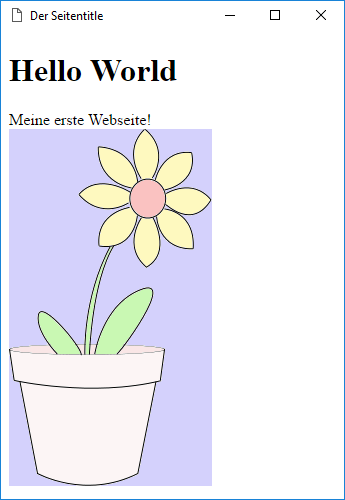
\includegraphics[width=.5\textwidth]{html.png}
        \caption{Beispiel HTML}
        \label{img:html}
    \end{center}
\end{figure}
\subsection{CSS}
\ac{css} bietet weitere Möglichkeiten zur Gestaltung von HTML-Dokumenten. Deren neueste Version, CSS3, befindet sich momentan in der Entwicklung, wird aber bereits jetzt von vielen Browsern verstanden. Die mit HTML beschriebenen Webseiten werden mit CSS in ihrer Erscheinung gestaltet und Dinge wie Farben und Breiten definiert. Man könnte z. B. das \autoref{lst:html} dahingehend erweitern, dass die Überschrift eine gelbe Hintergrundfarbe erhält, der darunter befindliche Text größer ist und das Bild kleiner dargestellt wird. Dies wird in \autoref{lst:css} gezeigt.

\begin{lstlisting}[style=htmlcssjs, caption=Beispiel CSS, label=lst:css]
<!DOCTYPE HTML>
<html>
  <head>
    <title> Der Seitentitle </title>
    <style>
      h1 {background-color:yellow}
      div {font-size:30pt}
      img {width:75; height:130 px;}
    </style>
  </head>
  <body>
    <h1> Hello World </h1>
    <div id="inhalt">Meine erste Webseite!</div>
    <img src="flowerpot.png" alt="Eine Blume" />
  </body>
</html>
\end{lstlisting}

Im Webbrowser dargestellt sieht \autoref{lst:css} aus wie in \autoref{img:css}.

\begin{figure}[H]
	\begin{center}
		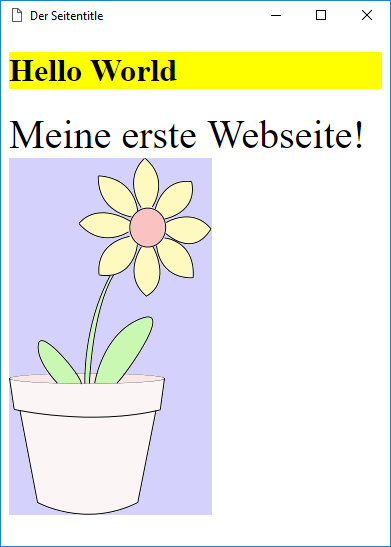
\includegraphics[width=.5\textwidth]{css.png}
		\caption{HTML erweitert mit CSS}
		\label{img:css}
	\end{center}
\end{figure}

Die Zeilen 6-8 in \autoref{lst:css} heißen CSS-Anweisungen. Der linke Teil ist der Selektor und gibt an, welche Elemente von der Regel betroffen sind. Der rechte Teil innerhalb der geschweiften Klammern ist die Deklaration. Diese besteht wiederum aus Paaren von Eigenschaften und Werten. Eigenschaft und Wert sind durch einen Doppelpunkt getrennt. Die Paare sind durch ein Semikolon getrennt. Mehrere CSS-Anweisungen ergeben zusammen ein Stylesheet.
\subsection{JavaScript}
JavaScript\index{JavaScript} ist eine Programmiersprache, die beim Ausführen, also z. B. beim Aufruf einer Webseite, von einem entsprechenden Programm interpretiert wird, und sie zählt somit zu den Interpreter-Sprachen. Zudem ist es eine schwach typisierte Sprache, das heißt, einer Variablen wird nicht explizit ein Typ zugewiesen, sondern sie erhält diesen implizit durch seinen Wert.
JavaScript wurde für den Einsatz innerhalb von Webseiten entworfen, wird heutzutage aber auch auf Servern verwendet. So werden Module für Node.js (\autoref{sec:nodejs}) in JavaScript geschrieben.\\
Bei JavaScript handelt sich um eine Implementation von ECMAScript\index{ECMAScript}, welche von Ecma International unter der Bezeichnung ECMA-262  spezifiziert wird, und sie wurde im Juni 2016 in der mittlerweile siebten Version veröffentlicht \cite{International2016}. Neuere Versionen bieten Sprachkonstrukte wie Module, Klassen und vieles mehr an. Jedoch unterstützen die Browser oder besser gesagt deren Interpreter bis dato nicht alle neuen Funktionen, wie \autoref{tab:ecmasupport} zu entnehmen ist. \\
\begin{minipage}{\textwidth}
\begin{longtable}{|c||c|c|c|}
	\hline  
	\backslashbox{\thead{Browser}}{\thead{Version}}& \thead{ECMAScript 5} & \thead{ECMAScript 6} & \thead{ECMAScript 7} \\  \hhline{|=||=|=|=|}
	\thead{Chrome 51} & 98 \% (Seit CH23+) & 98 \%  & 25 \% \\ 
	\hline 
	\thead{Firefox 47} & 100 \% (Seit FF21+) & 90 \% & 29 \% \\ 
	\hline 
	\thead{Safari 9} & 96 \% (Seit SF6+) & 53 \% & 1 \% \\ 
	\hline 
	\thead{Edge 13} & 99 \% (Seit IE10+) & 79 \% & 7 \% \\ 
	\hline 
	\thead{Android Browser 5.1} & 98 \% (Seit AN 4.4+)  & 29 \% & 4 \% \\ 
	\hline 
	\thead{iOS Safari 9} & 96 \% (Seit SF6+) & 53 \% & 1 \%\\ 
	\hline
	\caption{Ausschnitt der Browserunterstützung von ECMAScript \cite{ecmasupport}}\label{tab:ecmasupport}
\end{longtable}
\end{minipage}

Zu erkennen ist, dass gängige Browser in ihrer aktuellen Version weder Version 6 noch Version 7 zuverlässig unterstützen, wohingegen ECMAScript 5 in den meisten Browsern seit geraumer Zeit großteils lauffähig ist. Soll auch älteren Browsern der Zugriff auf eine Webpräsenz gewährleistet werden, so sollte man auf den Standard ECMAScript 3 aus dem Jahr 1999 zurückgreifen, da alle in \autoref{tab:ecmasupport} diese zu mindestens 96 \% unterstützen.\\
Zu beachten ist, dass in dieser Arbeit JavaScript als Synonym für ECMAScript steht. JavaScript ist lediglich eine Implementierung von ECMAScript der Organisation Mozilla Foundation. Jedoch werden aus geschichtlichen Gründen heute beide Begriffe oft als Synonym gehandhabt.

Mit JavaScript ist es möglich, auf Eingaben und Interaktionen des Anwenders zu reagieren und das Erscheinungsbild der Webseite dynamisch, ohne dass diese komplett neu geladen werden muss, zu verändern. Dies erfolgt durch Manipulation des \ac{dom}\index{DOM}, wobei es sich um eine Schnittstelle für den Zugriff auf ein HTML-Dokument handelt. Über die Schnittstelle lassen sich Knoten in einer Baumstruktur ablegen. Die durch das \autoref{lst:html} generierte HTML-Seite würde wie folgt aussehen.
\begin{figure}[H]
    \begin{center}
        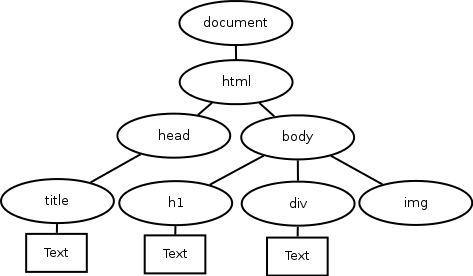
\includegraphics[width=.8\textwidth]{dom.png}
        \caption{Vereinfachte Baumstruktur des DOM ohne Attribute}
        \label{img:dom}
    \end{center}
\end{figure}

Der JavaScript-Code befindet sich innerhalb des HTML-Dokumentes in einem Script-Element, oder er wird als externe JavaScript-Datei in das HTML-Dokument eingebettet. Im folgenden Codebeispiel soll gezeigt werden, wie man ein Dokument mittels DOM-Manipulation beeinflussen kann.

\begin{lstlisting}[style=htmlcssjs, caption=Ein JavaScript Beispiel, label=lst:javascript]
<script>
  document.getElementById("inhalt").innerHTML="Ein neuer, Text!";
</script>
\end{lstlisting}

Es wird im Dokument aus \autoref{img:html} das Element mit dem id-Attribut und dem Wert \quotes{inhalt} gesucht und dessen Inhalt ersetzt. Der Text \quotes{Meine erste Webseite!} lautet nun: \quotes{Ein neuer Text!}. Zur DOM-Manipulation gehört auch die Möglichkeit, Elemente zu löschen, neue einzufügen und deren Attribute zu bearbeiten.\\
\subsection{TypeScript}
Bei TypeScript\index{TypeScript} handelt es sich um eine von Microsoft entwickelte Programmiersprache. Diese lehnt sich an ECMAScript Version 6 an. TypeScript erweitert deren Funktionsumfang aber um neue Elemente.\\ 
Jedoch unterstützten die Browser aus \autoref{tab:ecmasupport} kein TypeScript und können dieses nicht ausführen. Hierfür wird eine Anwendung benötigt, welche TypeScript in ECMAScript übersetzt. Solch eine Anwendung, genannt Transpiler\index{Transpiler}, stellt unter anderem Microsoft zur Verfügung und übersetzt TypeScript wahlweise in ECMAScript 5 bzw. ECMAScript 3 \cite[S. 439 f.]{ste15}. Ein Transpiler ist ein Programm, das eine Programmiersprache in eine andere übersetzt. So ist einem Entwickler die Möglichkeit gegeben die Vorteile von ECMAScript 6, wie Klassen und Vererbung, zu nutzen. Zudem ist es in TypeScript, im Gegensatz zu JavaScript, möglich, Variablen einem Typ zuzuweisen, womit diese auch stark typisiert genutzt werden können.
\subsection{Webserver}
\label{sec:webserver}
Die Entwicklung einer Webpräsenz ist prinzipiell auch ohne einen Webserver denkbar. Wird dieser lokal im Browser geöffnet, würde dies aber bei einem Ajax Aufruf, siehe hierzu \autoref{sec:ajax}, mit bei der Standardeinstellung gewisser Browser zu einem Same Origin Policy-Fehler führen \cite[S. 45  f.]{ste15}.\\
Abhilfe schafft hier der Einsatz eines Webservers. Als Plattform stehen neben dem Apache HTTP Server, nginx oder dem Microsoft Webserver ein auf Node.js basierender Webserver zur Auswahl. Dieser wird in \autoref{sec:nodejs} näher erläutert. \\
Zudem wird ein Webserver für den Produktiveinsatz benötigt, um Besuchern den Zugriff mit einem Webbrowser zu erlauben.
\subsection{URL}
\label{sec:url}\index{URL}
Ein \acf{url} identifiziert und lokalisiert eine Ressource. In der Webtechnologie verweist eine \ac{url} auf eine Web-Ressource. \\
Eine \ac{url} setzt sich aus verschiedenen Teilen, wie das verwendete Protokoll\index{Protokoll}, den Port\index{Port} und dem Hostname \index{Hostname} zusammen. Eine \ac{url} kann hierbei wie folgend aussehen.

\begin{lstlisting}[style=jcr, caption=Eine URL, label=lst:url]
http://www.example.com:3000/spa/index.html?page=news
\end{lstlisting}

Die \ac{url} aus \autoref{lst:url} in \autoref{tab:url} erklärt.

\begin{longtable}{|*6{c|}} 
	
	
	\hline 
	http & www & example.com & 3000 & spa/index.html & page=news\\ 
	
	\hline 
	 & Subdomain\index{Subdomain|see{Domain Subdomain}} & Domain\index{Domain} & & & \\
	\hline 
	Schema/Protokoll & \multicolumn{2}{c|}{Hostname} & Port & Pfad & Parameter\\
	\hline
	\caption{Aufbau einer URL}\label{tab:url}
\end{longtable}
\subsection{Servlet}
Bei einem Java-Servlet, kurz auch Servlet, handelt es sich um einen Java-Code, der auf einem Webserver ausgeführt wird \cite[S. 93]{Wissmann2012}. Diese nehmen Anfragen von Clienten entgegen und beantworten diese mit dynamisch generierten Nachrichten. Diese Nachrichten können zum Beispiel HTML-Seiten sein, welche zum Erstellen von serverseitigen Webanwendungen, siehe \autoref{sec:server-webanwendung}, genutzt werden können.
\subsection{HTTP}
\label{sec:http}\index{HTTP}

Beim \ac{http} handelt es sich um ein zustandsloses (Netzwerk-)Protokoll zur Datenübertragung, dessen Haupteinsatzgebiet im Internet ist. Ein Protokoll\index{Protokoll} definiert, wie Nachrichten in einem verteilten System untereinander verschickt werden. Eine Nachricht besteht in der Regel aus Metainformationen, welche sich im Header\index{Header} (eng. für Kopf) befinden, und den Nutzdaten.\\
Über \ac{http} werden Web-Ressourcen von einem Server zu einem Webbrowser übertragen. Hierbei kommunizieren der Webserver und der Webbrowser über das Protokoll. Der Ablauf erfolgt in etwa wie in \autoref{img:http-simple}.

\begin{figure}[H]
	\begin{center}
		\includesvg[width=0.5\textwidth]{http-simple}
		\caption{Kommunikationsbeispiel mit HTTP}
		\label{img:http-simple}
	\end{center}
\end{figure}


Der Client fordert vom Server, dem der Hostname www.example.com zugewiesen ist, die gewünschte Web-Ressource, hier index.html, an. Zusätzlich wird die gewünschte HTTP-Methode, hier GET, und die HTTP-Version, hier 1.1, definiert. Weiterhin ist das Versenden weiterer Parameter möglich. Diese Anfrage wird auch HTTP-Request\index{HTTP!HTTP-Request} genannt. Anschließend antwortet der Server im Erfolgsfall mit der angeforderten Web-Ressource und weiteren Metainformation, im Fehlerfall mit einem entsprechenden Statuscode. Die Antwort des Servers nennt sich HTTP-Response\index{HTTP!HTTP-Response}.\\
Im Normalfall besteht eine Webseite aber nicht nur aus einer HTML-Seite, sondern noch aus weiteren Ressourcen. Diese werden, zumindest in der HTML-Version 1.1, in etwa wie in \autoref{img:http} übertragen. Zu beachten ist, dass diese und folgenden Abbildungen im Gegensatz zur \autoref{img:http-simple} vereinfacht wurden und bewusst auf Informationen wie die HTTP-Methode und die HTTP-Version verzichtet wird.

\begin{figure}[H]
	\begin{center}
		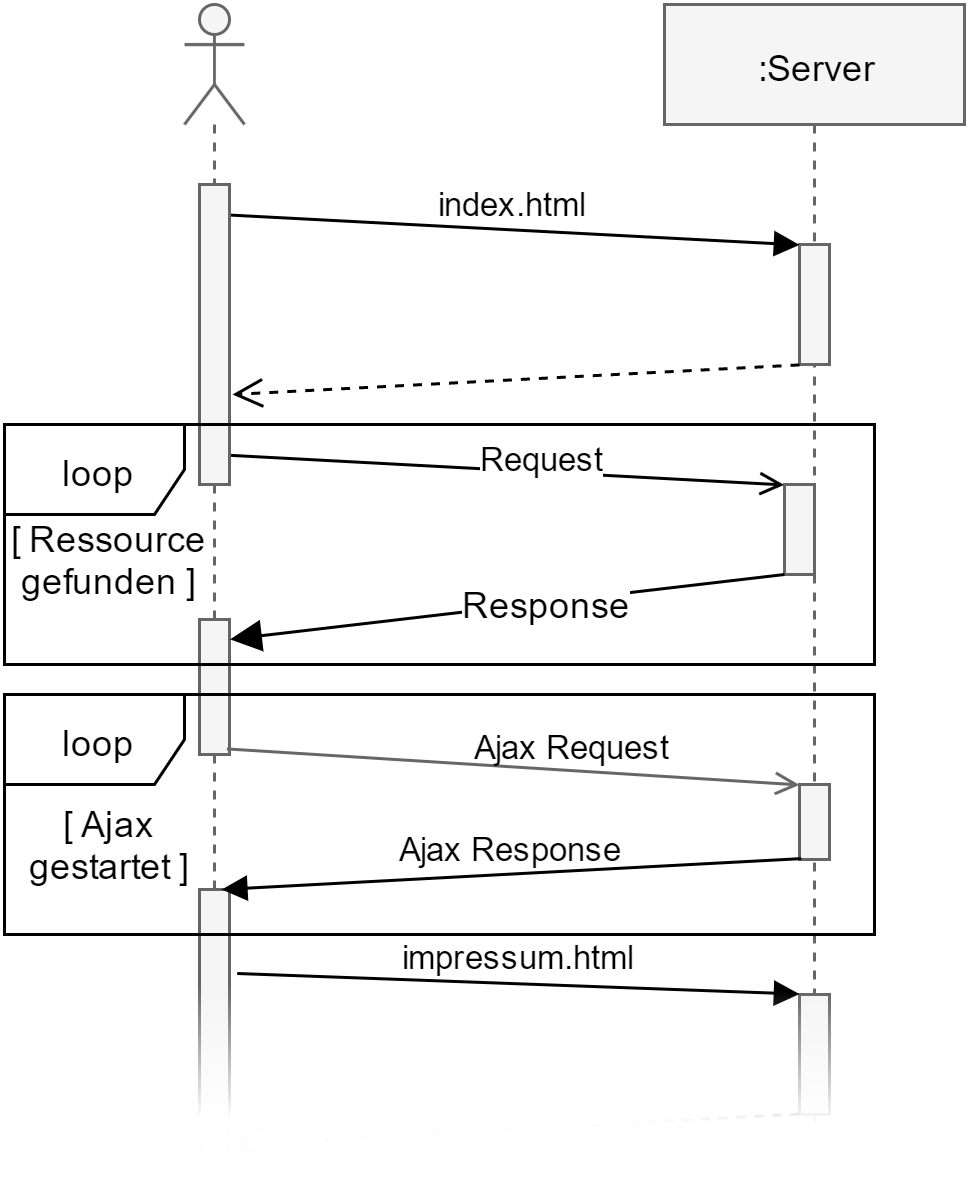
\includegraphics[width=0.5\textwidth]{http.png}
		\caption{Ladevorgang einer Webseite}
		\label{img:http}
	\end{center}
\end{figure}

Zunächst wird die eigentliche Webseite, am Beispiel \autoref{img:http} wäre dies index.html, angefordert. Nachdem diese vollständig geladen ist, durchsucht der Webbrowser den erhaltenen Quellcode nach weiteren Web-Ressourcen, wie Grafiken, Skripte, Stylesheets etc. und fordert auch diese vom Webserver an. Dabei können mehrere Anfragen gleichzeitig ausgeführt werden. Der Webbrowser achtet aber darauf, dass unter anderem Skripte in der gleichen Reihenfolge ausgeführt werden, wie diese im Quellcode der Webseite auftauchen, auch wenn ein später auftauchendes kleines Skript früher vollständig geladen wurde als eine zuvor erscheinende Bibliothek, um Abhängigkeitsfehler zu vermeiden. Weitere Web-Ressourcen kann der Client nun über Ajax anfordern, siehe hierzu \autoref{sec:ajax}. \\
Möchte der Benutzer nun die Webseite wechseln, zum Beispiel nach impressum.html, würde sich der Prozess entsprechend, gegebenenfalls mit anderen Ressourcen, wiederholen. \\
Einfach ausgedrückt, wird eine Webseite also wie folgt geladen.

\begin{description}
	\item[1. HTML-Seite:] Die darzustellende HTML-Seite wird vom Server angefordert.
	\item[2. Web-Ressourcen:] Der Quellcode der HTML-Seite wird nach weiteren Web-Ressourcen, wie Grafiken, Skripte oder Stylesheets, durchsucht und diese werden geladen.
	\item[3. Ajax:] Ajax Anfragen werden ausgeführt.
\end{description}

Eine Erweiterung von \ac{http} wäre das \ac{https}\index{HTTP!HTTPS}. Dieses ermöglicht zusätzlich eine verschlüsselte Kommunikation.
\subsection{Ajax}
\label{sec:ajax}\index{Ajax}
Durch die Verwendung von JavaScript lässt sich das Konzept von \ac{ajax} bewerkstelligen. Unter Zuhilfenahme dieses Konzeptes lassen sich neue Inhalte von einem Server nachladen, ohne die bestehende Seite neu zu laden. Dafür wird ein HTTP-Request an den Webserver gestellt, welcher mit den entsprechenden Daten antwortet. Diese erhaltenen Daten können anschließend durch DOM-Manipulation in die Seite eingebettet werden. Dies senkt sowohl die Ladezeit als auch das zu ladende Volumen an Daten. \\
Besagte Daten werden häufig, wie man vom Namen schon ableiten kann, im XML-Format übertragen. Andere Formate, wie z. B. JSON, sind jedoch auch möglich.
\subsection{XML und JSON}
Bei der \ac{xml}\index{XML} handelt es sich um eine Notation, um Daten hierarchisch und strukturiert in einer Textdatei und in einem für den Menschen lesbaren Format darzustellen \cite[S. 34]{seb10}. Als Beispiel soll eine kurze Datenbank für Musikstücke im \autoref{lst:xml} dienen. Diese besteht aus vier Musikstücken mit jeweils einer ID, einem Titel und einem Preis.
\begin{lstlisting}[style=xml, caption=Ein XML-Beispiel, label=lst:xml]
<?xml version="1.0" encoding="UTF-8" ?>
<songs>
	<song>
		<id>1</id>
		<title>Lets Go</title>
		<price>0.99</price>
	</song>
	<song>
		<id>2</id>
		<title>Song about Pencils</title>
		<price>2.3</price>
	</song>
	<song>
		<id>3</id>
		<title>Samba samba</title>
		<price>0.5</price>
	</song>
	<song>
		<id>4</id>
		<title>Another Song</title>
		<price>3.33</price>
	</song>
</songs>
\end{lstlisting}

Ein anderes, ebenfalls verwendetes Übertragungsformat bei Ajax ist \ac{json}\index{JSON}. Diese ist im Gegensatz zu XML kompakter und lässt sich direkt in JavaScript umwandeln \cite[S. 658]{rie09}. So könnte die Musikdatenbank hier wie in \autoref{lst:json} aussehen.

\begin{lstlisting}[style=htmlcssjs, caption=JSON für eine einfache Musikdatenbank, label=lst:json]
[
	{ "id": 1, "title": "Lets Go", "price": 0.99 },
	{ "id": 2, "title": "Song about Pencils", "price": 2.3 },
	{ "id": 3, "title": "Samba samba", "price": 0.5 },
	{ "id": 4, "title": "Another Song", "price": 3.33 }
]
\end{lstlisting}

Zu beachten ist, dass \autoref{lst:json} keine 1:1-Umsetzung von \autoref{lst:xml} darstellt, sondern einen etwas anders hierarchischen Aufbau verwendet. Zudem geht die Information, dass es sich um Songs handelt, verloren. Die damit darstellbaren Daten sind jedoch identisch.
\section{Fachliche Grundlagen}
Die zuvor beschriebenen Begriffsdefinitionen und technischen Grundlagen dienten dem Verständnis des folgenden Kapitels. \\ 
Nun sollen auch einige Grundlagen erklärt werden, um das Thema dieser Arbeit besser verstehen zu können.
\subsection{Webanwendung}
\label{sec:webanwendung}\index{Webanwendung}
Frühere Webpräsenzen waren meist recht simpel gestaltet. Traditionell waren dies oft einfache Plattformen, um statische Informationen über das Internet zu verteilen. Einzig bei der Navigation durch die einzelnen Webseiten erfolgte eine Interaktion mit dem Besucher. Der Client schickt an den Webserver eine Anfrage, welche Webseite er gerne hätte, und erhält als Antwort das HTML-Dokument, siehe \autoref{img:http-website}.

\begin{figure}[H]
	\begin{center}

		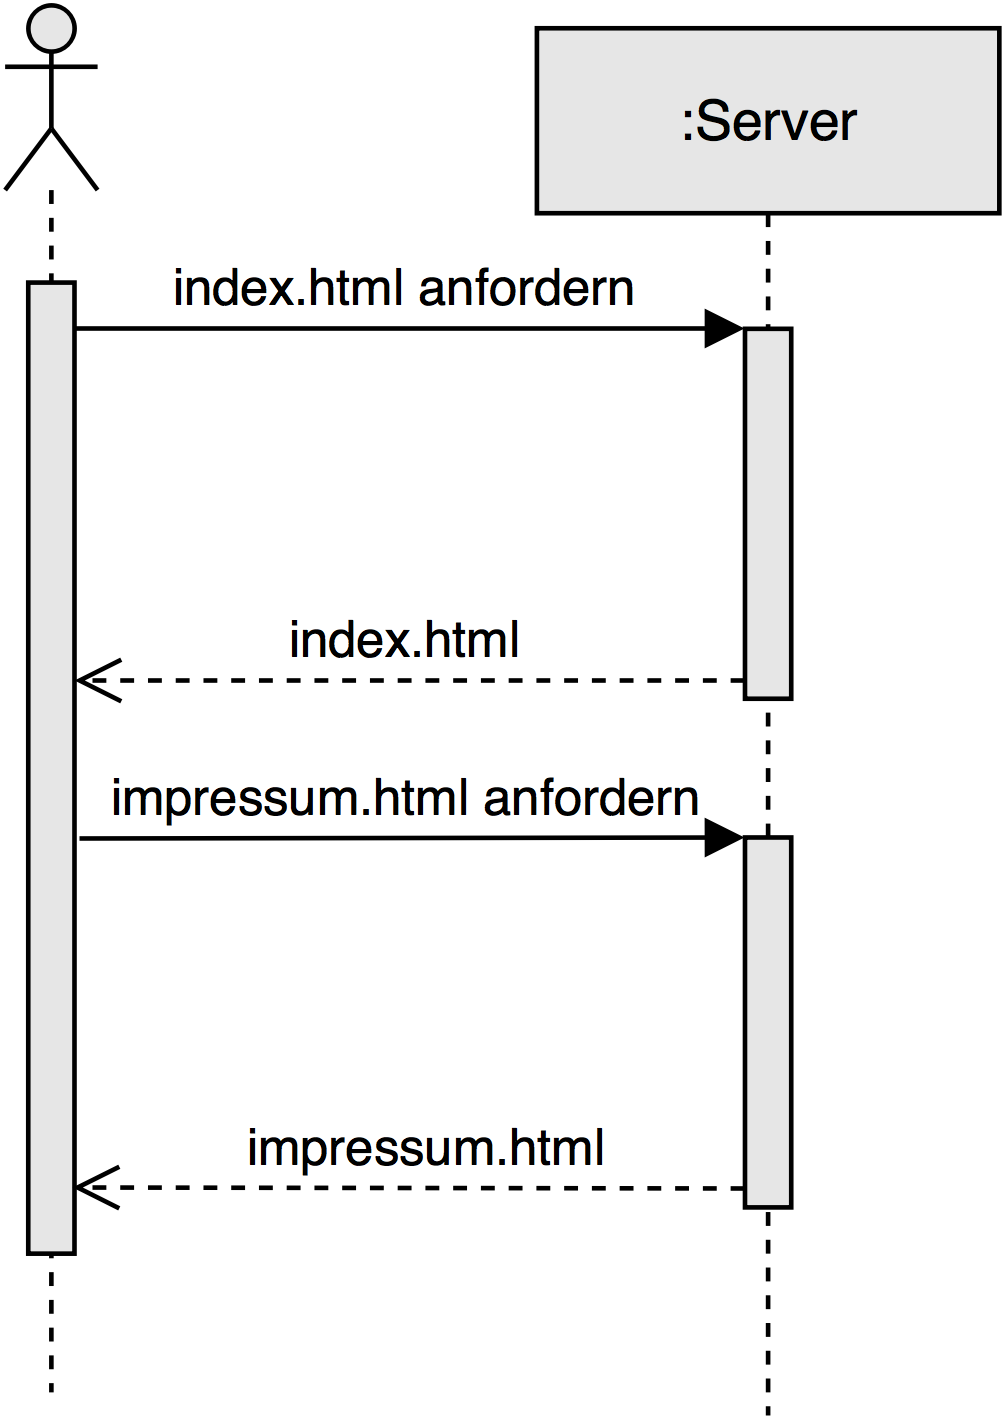
\includegraphics[width=.3\textwidth]{http-request.png}
		\caption{Systematischer Ablauf beim Abruf von Webseiten}
		\label{img:http-website}
	\end{center}
\end{figure}

Erst durch den Onlinehandel, webbasierte Buchungssysteme und Online-Auktionssysteme entstanden die ersten Webanwendungen als Weiterentwicklung von Webpräsenzen. Hierbei interagiert der Besucher neben der klassischen Navigation noch auf anderen Wegen mit der Webanwendung. So kann dieser zum Beispiel bei einem Onlinehändler für Musik durch die einzelnen Webseiten navigieren, durch entsprechende Anfragen das Musikangebot nach seinen Interessen filtern und Musikstücke erwerben \cite[S. 89]{lid00}. \\
Ein wesentlicher Unterschied zu Softwareanwendungen ist hier, dass eine Webanwendung mithilfe von Techniken und Standards, unter anderem vorgeschlagen vom \ac{w3c}, entwickelt wird und so Web-Ressourcen über einen Webbrowser bereitstellt \cite[S. 2]{kap03}.

\input{inhalt/grundlagen/fachliche-grundlagen/webanwendung/Serverseitige-und-Clientseitige-Webanwendungen}

\input{inhalt/grundlagen/fachliche-grundlagen/webanwendung/Single-Page-Webanwendung}
\subsection{Framework / Bibliothek}
Eine Bibliothek\index{Bibliothek} ist eine Codesammlung, mir der sich wiederkehrende Codestrukturen abbilden lassen, um einen kürzeren und stabileren Quellcode zu verfassen. Ein Framework\index{Framework} liefert zudem noch ein  Programmiergerüst, welches vorgefertigte Funktionalitäten mitbringt. Dieses Gerüst liefert den Rahmen (Frame), innerhalb dessen sich Anwendungen erstellen lassen. Ein Framework legt im Gegensatz zu einer Bibliothek auch eine Steuerung von Verhaltensweisen bei der Verwendung fest \cite[S. 20]{steyer2011jquery}.  Eine Art solcher Frameworks sind Webframeworks. Mit diesen lassen sich Webanwendungen entwickeln. In Rahmen dieser Arbeit sind z. B. die Webframeworks AngularJS, AngularJS2, React und Aurelia, siehe \autoref{sec:auswahl-und-bewertung}, relevant.
\subsection{MV*-Architekturmuster}
Häufig unterstützen Webframeworks, aber auch diverse Content Management-Systeme, verschiedene Architekturmuster, um die Entwicklung von Webanwendungen modularer zu gestalten. Der Gedanke dabei ist es, den Quellcode zum Beispiel in Logik und Präsentation aufzuteilen. So ist der Code für Entwickler leichter zu warten, die Testbarkeit verbessert sich und es ergeben sich wiederverwendbare Codestücke \cite[S. 34]{ste15}. \\
Eines dieser Entwurfsmuster ist das \ac{mvc}\index{MVC}. Dieses besteht aus drei Komponenten. Wie diese interagieren, beschreibt \autoref{img:mvc}.

\begin{figure}[H]
	\begin{center}
		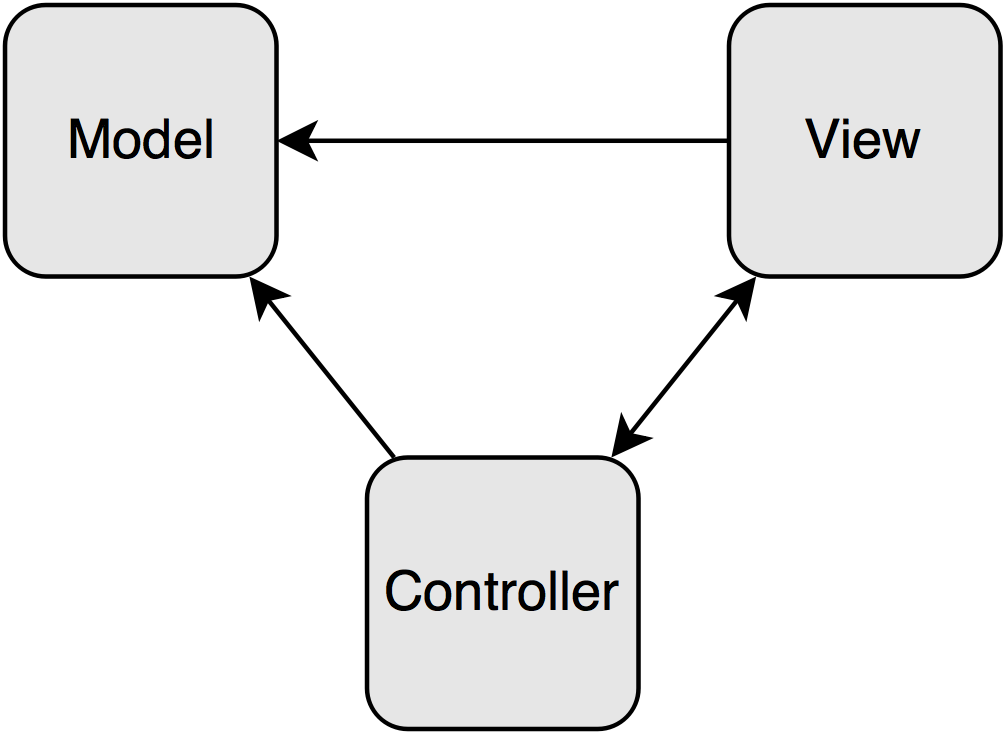
\includegraphics[width=.6\textwidth]{mvc.png}
		\caption{MVC-Muster}
		\label{img:mvc}
	\end{center}
\end{figure}

Die Model-Komponente\index{Model} beinhaltet die darzustellenden Daten. In der View-Komponente\index{View} wird beschrieben, wie die Daten darzustellen sind. Die Controller-Komponente\index{Controller} regiert auf Benutzeraktionen und beeinflusst die Darstellung der View und die Daten des Models. Zudem können beim \ac{mvc} komplexere Views in mehrere einzelne Views aufgeteilt und ineinander verschaltet werden \cite[S. 5 ff.]{gof}.

Als weiteres Entwurfsmuster ist das \ac{mvvm}\index{MVVM} zu nennen. Model und View entsprechen dem des \ac{mvc}-Musters. Anstelle eines Controllers wird hier aber ein View-Model\index{View-Model} eingesetzt. Hier wird die Logik der Bedienoberfläche (View) beschrieben und referenziert zu den Daten (Model) \cite[S. 40]{mvvm}, vergleiche \autoref{img:mvvm}. Im Gegensatz zum Controller im \ac{mvc}-Muster besitzt das View-Model hier keinerlei Informationen über die View. Dies erleichtert den Austausch der View und erlaubt, dass sich mehrere Views auf ein View-Model beziehen.

\begin{figure}[H]
	\begin{center}
		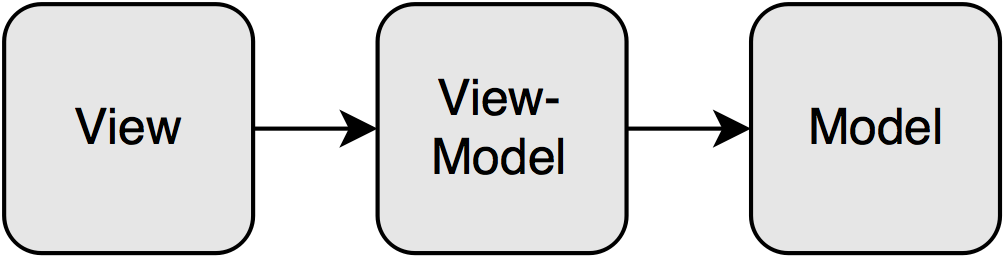
\includegraphics[width=.6\textwidth]{mvvm.png}
		\caption{MVVM-Muster}
		\label{img:mvvm}
	\end{center}
\end{figure}

Bei MV*-Architekturmustern wird die View häufig durch ein oder mehrere Templates (Vorlagen)\index{Template} beschrieben. Im Zusammenhang mit MV* ist ein Template eine Vorlage für das Aussehen einer Webseite, in dem wiederkehrende Elemente definiert werden. Diese werden für gewöhnlich in separaten Dateien gespeichert und mit Platzhaltern und einer einfachen Logik versehen. Anhand der Daten des Models und ggf. weiterer Variablen werden die Platzhalter gefüllt und so ein HTML-Dokument erstellt, das dem Clienten zugeschickt wird. Die semantische Darstellung der Platzhalter und des Logikflusses ist von der verwendeten Templatesprache abhängig \cite[S. 37]{newman2008django}.
\subsection{Content Management System}

Unternehmen verwenden Webpräsenzen, um sich online zu präsentieren. Dabei liegt der Fokus des Managements darauf, Informationen schnell und aktuell dem Kunden zur Verfügung zu stellen. Um dies zu erreichen, werden \acf{cms} verwendet. Diese erleichtern die Trennung von Inhalt (z.B. Texte, Bilder, Videos etc.), Layout und Struktur \cite[S.1 ff.]{spo09}. Somit muss sich ein Redakteur nicht mit dem Aussehen der Webpräsenz beschäftigen und kann sich nur auf den Inhalt fokussieren. \\
Ein \ac{cms} bietet zumeist eine Vielzahl an Funktionalitäten. Dazu gehören das Erstellen und Strukturieren von Inhalten, eine Mehrbenutzerfähigkeit und administrative Funktionen zum Verwalten besagter Nutzer \cite[S. 55]{spo09}.  Die Verwendung erfolgt über eine grafische Bedienoberfläche, um den Umgang mit dem System auch technisch weniger affinen Menschen zu vereinfachen. Diese ist generell über einen Webbrowser aufzurufen und zu verwenden. Somit benötigt ein Autor keine Zusatzsoftware und kann ortsungebunden arbeiten \cite[S. 19 f.]{bon11}.

\input{inhalt/grundlagen/fachliche-grundlagen/content-management-system/Adobe-Experience-Manager}


\chapter{Webframeworks}
\label{sec:webframeworks}
Um die Komplexität einer \ac{spa} zu bewältigen, haben sich in den vergangenen Jahren Teams von Entwicklern mit dem Ziel zusammen getan, Webframeworks zu entwickeln, um auf deren Grundlage die Entwicklung künftiger \ac{spa}s zu vereinfachen. \\
Folgend soll zunächst auf Werkzeuge und Techniken eingegangen werden, deren Einsatz in allen Webframeworks möglich ist. Anschließend folgt eine Auflistung von Eigenschaften, die ein Webframework mitbringen sollte, damit sich eine Neuentwicklung einer \ac{spa} hiermit lohnt. Anschließend wird eine Auswahl an Webframeworks genannt und näher erläutert.

\section{Werkzeuge und Techniken}
Die Entwicklung einer Webanwendung wird durch den richtigen Einsatz entsprechender Werkzeuge vereinfacht und automatisierte Vorgänge werden zum gegebenen Zeitpunkt ausgeführt. Folgend werden einige Werkzeuge samt entsprechenden Beispielprogrammen gelistet.

\subsection{Node.js}
\label{sec:nodejs}\index{Node.js}

Node.js ermöglicht es serverseitige Webanwendungen in JavaScript zu verfassen \cite[S. 4]{Fedosejev2015}. Weiterhin können auch clientseitige Webanwendung hiermit zugänglich gemacht werden. Node.js bietet eine Erweiterung an, welche TypeScript automatisiert in JavaScript umwandelt. Dies beschleunigt die Entwicklung von in TypeScript verfassten Webanwendungen, da eine Umwandlung bei Änderung des Quellcodes nicht manuell angestoßen werden muss.
\subsection{Paketverwaltung}
Für Node.js gibt es ein breites Spektrum an Erweiterungen. Zur Verwaltung dieser Erweiterungen existiert der \ac{npm}, welches derzeit über 330.000 Pakete umfasst \cite{DeBill2016}. Unter anderem wird so die einfache Installation von Werkzeugen für die Entwicklung oder auch das Laden von JavaScript-Bibliotheken und Frameworks ermöglicht. Alternativ kann über \ac{npm} auch die Installation anderer Paketverwaltungs-Programme wie Bower \cite{bower.io} erfolgen. 
\subsection{Automatisierungswerkzeuge}
\label{sec:automatiserungswerkzeuge}
Oft muss eine Webanwendung, sobald diese in ihre produktive Umgebung überführt wird, einigen Anpassungen unterliegen. Hierzu zählen Dinge wie die Minimierung von Quellcode, Anpassen von Pfaden oder Konkatenieren von Dateien. Damit dies nicht der Entwickler händisch übernehmen muss und sich dabei mögliche Flüchtigkeitsfehler einschleichen, existieren speziell für JavaScript als Anwendungen entworfene Werkzeuge für die Automatisierung. Als populäre Beispiele hierfür wären Grunt \cite{gruntjs.com} und Gulp \cite{gulpjs.com} zu nennen \cite[S. 246 f.]{ste15}.
\subsection{Modularisierung und Verwaltung von Abhängigkeiten}
Nicht selten besitzt ein Codestück Abhängigkeiten zu anderen Programmcodes, damit dieses korrekt funktioniert. Dies sind zum Beispiel Bibliotheken, Frameworks oder Codestücke von anderen Entwicklern. Zu gewährleisten, dass alle diese Abhängigkeiten korrekt aufgelöst werden, mag bei kleinen Projekten noch ohne Weiteres vom Entwickler allein zu bewältigen sein. Hierfür muss er alle Skripte in der korrekten Reihenfolge in das HTML-Dokument einbinden. Sobald ein Projekt aber wächst und mehrere Entwickler daran beteiligt sind, steigt auch die Komplexität und somit auch die Herausforderung, besagte Abhängigkeiten aufzulösen. \\
Lösungen hierfür sind Entwurfsmuster wie \ac{di}, \ac{ioc} \cite[S. 25 ff.]{GollDausmann2013} oder das Entwickeln gegen Schnittstellen, wie der \ac{amd} \cite[S. 266 ff.]{ste15}. Das Ziel ist dabei, den Code zu modularisieren, die Entkopplung von Abhängigkeiten und eine komponentenorientierte Entwicklung \cite[S. 261]{ste15}. Für die Zusammenführung der einzelnen Module haben sich gewisse Bibliotheken etabliert. Eine Zusammenfassung der derzeit bedeutendsten Bibliotheken und für welche Art von Modulen diese geeignet sind, ist \autoref{tab:dilist} zu entnehmen.

\begin{minipage}{\textwidth}
\begin{longtable}{|c|c|}
	\hline  
	\thead{Bibliothek} & \thead{Geeignet für}\\  \hhline{|=|=|}
	browserify &  npm-Module \\
	\hline
	RequireJS & ES 2015 Module, \ac{amd}   \\ 
	\hline 
	SystemJS &  ES 2015 Module, \ac{amd}, CommonJS  \\ 
	\hline 
	Webpack & CommonJS, \ac{amd}   \\ 
	\hline 
	
	\caption{Möglichkeiten für Dependency Injection}\label{tab:dilist}
\end{longtable}
\end{minipage}


In jedem Modul wird deklariert, welche anderen Modulabhängigkeiten dieses besitzt. Die Syntax jener Deklaration ist von dem genutzten Entwurfsmuster bzw. der genutzten Schnittstelle abhängig. Die verwendete Bibliothek löst die Abhängigkeiten auf und übergibt den Modulen Instanzen ihrer benötigten Module. 


\section{Anforderungen}
\label{sec:anforderungen_webframeworks}

Bei der Integration der Frameworks gilt es, gewisse Faktoren zu berücksichtigen. Dies sind Anforderungen, die ein Framework erfüllen muss, um einen langfristigen und zufriedenstellenden Einsatz gewährleisten zu können. Zudem müssen bei der Integration der final entwickelten Webanwendung einige Punkte Beachtung finden. \\
Die Vorgaben sind zumeist von extern, also von Kunden, und werden im Folgenden nicht immer erläutert, warum diese so und nicht anders ausgefallen sind. 

\subsection{Browserunterstützung}
Da die Webanwendungen bei möglichst vielen Besuchern lauffähig sein sollen, ist die Browserunterstützung hier ein wichtiger Aspekt. \\ Die Mindestversion der Browser ist \autoref{tab:browsersupport} zu entnehmen.

\begin{minipage}{\textwidth}
\begin{longtable}{|c|c|c|}
	\hline  
	\thead{Browser} & \thead{Mindestversion} & \thead{Veröffentlicht am}\\  \hhline{|=|=|=|}
	
	Chrome & 23 & 25.09.12 \\ 
	\hline 
	Firefox & 16 & 28.08.12 \\ 
	\hline 
	Safari & 6 & 25.07.12\\ 
	\hline 
	Internet Explorer / Edge & 10 & 04.09.12 \\ 
	\hline 
	Android Browser & 4.4 & 09.12.13\\ 
	\hline 
	iOS Safari & 6.1 & 28.01.13 \\ 
	\hline 
	\caption{Browsersupport der Webanwendungen}\label{tab:browsersupport}
\end{longtable}
\end{minipage}

\subsection{Integration}

Die Autoren-Bedienoberfläche von \ac{aem} inkludiert bereits eine Reihe von JavaScript und CSS-Ressourcen. Diese sind vonnöten, um verschiedene Funktionalitäten, wie zum Beispiel die Konfiguration der Komponenten, zu gewährleisten. Es ist somit darauf zu achten, dass Skripte, die vom Framework, von der Webanwendung oder von der Integration der Webanwendung in das \ac{aem} stammen, nicht mit Skripten seitens \ac{aem} kollidieren.

%\subsection{Suchmaschinenoptimierung}
\subsection{Indizierung von Suchmaschinen}
\label{sec:seo}

Das Internet ist eines der sich am schnellsten entwickelnden Medienlandschaften. Viele Unternehmen unterschiedlichster Größenordnung sind hier vertreten, manch eine Firma präsentiert sich sogar nur online \cite[S. 29 f.]{EstherKessler2015}. Da viele Benutzer täglich eine Suchmaschine verwenden oder eine als Startseite ihres Browsers festgelegt haben, sollte es für ein Unternehmen von hoher Wichtigkeit sein, dass seine Webpräsenz mit den richtigen Begriffen bei einer Suche möglichst weit oben erscheint \cite[S. 147]{EstherKessler2015}.\\

\subsubsection{Funktionsweise einer Suchmaschine}
Damit eine Webpräsenz mitsamt ihren Webseiten überhaupt in einem Suchergebnis erscheint, werden diese von der jeweiligen Suchmaschine zunächst indiziert. Dies übernehmen Programme, sogenannte Crawler\index{Crawler} oder auch Robots\index{Robot|see{Crawler}}. Diese durchsuchen das Internet und erstellen einen Katalog aller gefundenen Webseiten. Weitere Webseiten werden über interne und externe Hyperlinks, die sich in den zuvor gefundenen Webseiten befinden, erreicht. Externe Hyperlinks sind eine Möglichkeit, weitere Webpräsenzen zu finden. Auch diese werden wieder indiziert und auf weitere Hyperlinks durchsucht. Solch eine Navigationsstruktur kann wie in \autoref{img:navi-mpa} aussehen.

\begin{figure}[H]
	\begin{center}
		\includegraphics[width=.8\textwidth]{navi-mpa.png}
		\caption{Mögliche Navigationsstruktur einer Webseite}
		\label{img:navi-mpa}
	\end{center}
\end{figure}

Zu sehen ist, dass alle Webseiten von der Einstiegsseite (\pseudourl{index.html}) aus zu erreichen sind. Über diese wird auf die Nachrichtenübersicht (\pseudourl{/news}) und das Impressum (\pseudourl{/abbout}) verwiesen. Die beiden Nachrichteneinträge (\pseudourl{/news/1989/07/01} und \pseudourl{/news/2014/04/01}) sind über die Nachrichtenübersicht erreichbar. Im Impressum ist ein externer Hyperlink (\pseudourl{kandler.li/index.php}) vorzufinden.

Anhand von Schlagwörtern und Algorithmen werden die Webseiten analysiert und in den Katalog der Suchmaschine aufgenommen. Besagter Algorithmus entscheidet, welche Webseite durch welche Suchbegriffe in der Reihenfolge der Suchergebnisse erscheint. Dieser Algorithmus ist in der Regel äußerst komplex und umfasst am Beispiel Google über 200 zu berücksichtigende Faktoren \cite[S.163 f.]{EstherKessler2015}. 

Nun sollte eine Suchmaschine in der Lage sein, eine Webpräsenz samt all ihrer Webseiten zu indizieren. Die Suche nach \quotes{www.example.com Impressum} sollte hier im Idealfall als erstes Ergebnis das Impressum von \pseudourl{example.com} liefern. \\

\subsubsection{Probleme bei Single-Page-Webanwendungen}
Nun ist eine \ac{spa} so gestaltet, dass diese nur aus einer einzigen HTML-Seite besteht und ein Nachladen von Inhalten meist durch JavaScript und \ac{ajax} erfolgt. Wegen dieser Eigenschaften resultieren einige Probleme in der Indizierung.


\paragraph{Nachladen mit JavaScript}

Suchmaschinen analysierten früher zur Indizierung lediglich den Quellcode einer Webseite. Alle JavaScript-Anweisungen wurden ignoriert und nicht wie in einem Webbrowser interpretiert, womit eine \ac{spa} für die Suchmaschine oft ohne bedeutenden Inhalt erschien. Im Jahr 2009 gab Google bekannt, nun auch JavaScript und \ac{ajax} beim Crawling zu berücksichtigen \cite{Google2009}.\\

\paragraph{Hyperlinks innerhalb der SPA}
Problematisch ist aber noch die Navigation zwischen den einzelnen Webseiten. Bei einer traditionellen \ac{mpa} geschieht dies durch Hyperlinks. Über z. B. \pseudourl{http://www.example.com} wäre die Startseite der Webpräsenz zu erreichen, über \pseudourl{http://www.example.com/news} alle Neuigkeiten und hinter \pseudourl{http://www.example.com/about} könnte sich das Impressum verstecken, wie zum Beispiel in \autoref{img:navi-mpa} zu sehen. Jede Unterseite würde von einer Suchmaschine korrekt indiziert werden. Ein Hyperlink innerhalb einer \ac{spa} wurde oft mit einer Sprungmarke \cite{Consortium2016}\index{Sprungmarke}, zu erkennen an der Raute (\#), versehen. Die Neuigkeiten wären nun über \pseudourl{http://www.example.com/index.html\#news} und das Impressum über \pseudourl{http://www.example.com/index.html\#about} zu erreichen. Die Navigationsstruktur aus \autoref{img:navi-mpa} würde nun wie in \autoref{img:navi-spa} aussehen.

\begin{figure}[H]
	\begin{center}
		\includegraphics[width=.8\textwidth]{navi-spa.png}
		\caption{Mögliche Navigationsstreukur in einer SPA}
		\label{img:navi-spa}
	\end{center}
\end{figure}

Alle Seiten einer \ac{spa} wurden von gängigen Suchmaschinen nur als eine Seite, also \pseudourl{http://www.example.com/index.html}, interpretiert. Bis Oktober 2015 empfahl Google, um dieses Problem zu umgehen, die Raute um ein Ausrufezeichen (!) zu ergänzen, womit sich ein Hyperlink der Form \pseudourl{http://www.example.com/\#!about} ergab. Der Crawler ersetzt nun die Zeichenkombination \quotes{\#!}, welche auch Shebang\index{Shebang} genannt wird, durch \quotes{?\_escaped\_fragment\_=}, was zu \ac{url}s wie zum Beispiel \pseudourl{http://www.example.com/?\_escaped\_fragment\_=about} führt. Der Crawler erwartet nun vom Server unter dieser \ac{url} eine reine HTML-Seite ohne JavaScript und mit den gleichen Inhalten, wie ein Besucher dies auch beim Aufruf von \pseudourl{http://www.example.com/\#!about} nach der Ausführung aller JavaScript-Anweisungen erhalten hätte.

\paragraph{Lösung durch die pushState-Funktion}
\label{sec:pushState}\index{pushState-Funktion}
Die Indizierung durch Einsatz von Shebang funktioniert zwar noch, wird aber seit Oktober 2015 von Google offiziell nicht länger empfohlen. Anstelle dieser sollen Techniken und Methoden der progressiven Verbesserung Verwendungen finden, um Webpräsenzen auch zukünftig zuverlässig indizieren zu können. Hierbei kann unter anderem die in HTML5 eingeführte JavaScript-Funktion pushState Verwendung finden \cite{Google2015}. Diese Funktion kann den Browserverlauf manipulieren und diesem einen neuen Eintrag hinzuzufügen, ohne einen neuen HTTP-Request auszulösen. Bei dieser Technik werden Hyperlinks wieder im traditionellen Format angelegt, also z. B. auf \pseudourl{http://www.example.com/about}. Zur Verdeutlichung des Ablaufes soll \autoref{img:pushState} dienen.

\begin{figure}[H]
	\begin{center}
		\includegraphics[width=.5\textwidth]{pushState.png}
		\caption{Ablauf des Webseitenwechsels in SPAs mit Verwendung der pushState-Funktion}
		\label{img:pushState}
	\end{center}
\end{figure}

Navigiert der Besucher nun von der Startseite auf das Impressum (\pseudourl{example.com/about}), wird der HTTP-Request abgefangen. Der benötigte Inhalt für das Impressum wird über \ac{ajax} geladen und in die Seite eingefügt. Im Anschluss wird durch die pushState-Funktion der Browserverlauf manipuliert. Nun ist der letzte Eintrag im Browserverlauf \pseudourl{http://www.example.com/news} und in der Adresszeile wird nun die vom Hyperlink angeforderte \ac{url} angezeigt. Für den Benutzer scheint es so, als ob er die alte HTML-Seite verlassen hätte und sich nun auf einer neuen befindet.\\
Nun muss der Webserver noch so konfiguriert werden, dass alle Anfragen, die mit der Basis-\ac{url} der \ac{spa} beginnen, auf selbige umgeleitet werden, damit ein direkter Aufruf, zum Beispiel von einer externen Seite, funktioniert. Sowohl \pseudourl{http://www.example.com/news} als auch \pseudourl{http://www.example.com/about} würde der Server nun auf \pseudourl{http://www.example.com/} weiterleiten. Die \ac{spa} würde nun den Zusatz der ursprünglich angeforderten \ac{url} \pseudourl{/news} bzw. \pseudourl{/about} erkennen und den entsprechenden Inhalt darstellen. Durch diesen Trick kann nun der Google Crawler jede Webseite einer \ac{spa} durch eine eindeutige \ac{url} erreichen. \\
Es ist somit darauf zu achten, dass das Framework korrekt von gängigen Suchmaschinen interpretiert wird und dass alle Webseiten durch Verwendung gültiger Links indiziert werden.

\subsection{Lizenz}
Da das Framework auch kommerziell genutzt werden soll, ist auch auf dessen Lizenz zu achten. Gängige Lizenzen, welche für eine kommerzielle Nutzung geeignet wären, sind zum Beispiel die 3-Klause-BSD- \cite{3rdclausebsd} und MIT-Lizenz \cite{mit}.
\section{Auswahl \& Bewertung}
\label{sec:auswahl-und-bewertung}

Die in diesem Kapitel genannten Frameworks, also AngularJS, AngularJS2, Aurelia und React, sollen im \autoref{sec:integration-der-webframeworks-in-aem} versucht werden in das \ac{aem} zu integrieren. Zu beachten ist, dass im Folgenden React gelegentlich auch als Framework betitelt wird, auch wenn es sich hier streng genommen um eine Bibliothek handelt. \\

\subsection{AngularJS}
\label{sec:angularjs}\index{AngularJS}
AngularJS ist ein von Google Inc. entwickeltes clientseitiges Webframework. Mit diesem lassen sich Webanwendungen und \ac{spa}s entwickeln. Für den Entwickler ist es zudem möglich verschiedene MV*-Architektur zu realisieren, was durch vorgegebene Richtlinien zum Erstellen von Views, Controller Models erbracht wird. Hierzu gehören sowohl die \ac{mvc}- als auch die \ac{mvvm}-Entwurfsmuster \cite{ste15}.

\input{inhalt/webframeworks/auswahl-und-bewertung/angularjs/Datenbindung}
\input{inhalt/webframeworks/auswahl-und-bewertung/angularjs/Module}
\input{inhalt/webframeworks/auswahl-und-bewertung/angularjs/Services}
\input{inhalt/webframeworks/auswahl-und-bewertung/angularjs/Dependency-Injection}
\input{inhalt/webframeworks/auswahl-und-bewertung/angularjs/Templates}
\input{inhalt/webframeworks/auswahl-und-bewertung/angularjs/Direktiven}
\input{inhalt/webframeworks/auswahl-und-bewertung/angularjs/Scope}
\subsection{AngularJS2}
\label{sec:angularjs2}\index{AngularJS2}

Zum Zeitpunkt dieser Arbeit ist Google Inc. dabei, den Nachfolger von AngularJS zu entwickeln, genannt AngularJS2. Hierbei handelt es sich um keine Weiterentwicklung von AngularJS, sondern es wird von Grund auf neu entwickelt.

\input{inhalt/webframeworks/auswahl-und-bewertung/angularjs2/Unterschied-zu-AngularJS}

\input{inhalt/webframeworks/auswahl-und-bewertung/angularjs2/Komponenten}

\input{inhalt/webframeworks/auswahl-und-bewertung/angularjs2/Performance}

\input{inhalt/webframeworks/auswahl-und-bewertung/angularjs2/Datenbindung}

%\begin{itemize}
%	\item Data-Binding ohne Dirty Checking http://blog.angular-university.io/introduction-to-angular2-the-main-goals/
%\end{itemize}


\subsection{Aurelia}
\label{sec:aurelia}\index{Aurelia}

Hauptverantwortlicher für das Framework Aurelia ist Rob Eisenberg. Dieser entwickelte bereits das JavaScript Framework Durandal und half bei der Entwicklung von AngularJS2 mit. Da dessen Entwicklung Eisenberg jedoch nicht zufrieden stellte, entschloss er sich, das Google-Team zu verlassen und erneut ein neues Framework unter dem Namen Aurelia zu kreieren \cite{Eisenberg2014}.

\input{inhalt/webframeworks/auswahl-und-bewertung/aurelia/Sprachen}

\input{inhalt/webframeworks/auswahl-und-bewertung/aurelia/Templates}

\input{inhalt/webframeworks/auswahl-und-bewertung/aurelia/Depency-Incetion}

\input{inhalt/webframeworks/auswahl-und-bewertung/aurelia/Support}

\subsection{React}
\label{sec:react}

Einen etwas anderen Ansatz verfolgt React. Es handelt sich bei dem von Facebook und Instagram entwickelten Code nicht um ein Framework, sondern um eine Bibliothek. 

\input{inhalt/webframeworks/auswahl-und-bewertung/react/virtueller-dom}
\input{inhalt/webframeworks/auswahl-und-bewertung/react/JSX}


\newpage
\subsection{Vergleich}

Folgende \autoref{tab:vergleich} zeigt kurz zusammengefasst die wichtigsten Eigenschaft der zuvor genannten Webframeworks im Vergleich. \\
\begin{minipage}{\textwidth}
\begin{longtable}{|c||p{0.15\textwidth}|p{0.15\textwidth}|p{0.15\textwidth}|p{0.15\textwidth}|}
	\hline  
	\backslashbox{\thead{Eig.}}{\thead{Webfr.}}& \thead{AngularJS} & \thead{AngularJS2} & \thead{Aurelia} & \thead{React} \\  \hhline{|=||=|=|=|=|}
	
	\thead{Entwurfsmuster} & MVC, MVVM & MVC, MVVM & MVC, MVVM  & keines \\ 
	\hline 
	\thead{Sprache} & JS & JS/TS & JS/TS & JS \\
	\hline
	\thead{Lizenz} & MIT & MIT & MIT & 3-Klause-BSD \\
	\hline
	\thead{Besonderheiten} & Datenbindung & Verbesserte Laufzeit & ESNext, Support & Shadow DOM\\
	\hline
	\thead{Entwickler} & Google & Google & Blue Spire & Facebook, Twitter \\
	\hline
	\thead{Webpräsenz} & \pseudourl{http://angularjs.org/} & \pseudourl{http://angular.io} & \pseudourl{http://aurelia.io} & \pseudourl{http://facebook.github.io/react/} \\
	\hline

	\caption{Vergleich der vier Frameworks}\label{tab:vergleich}
\end{longtable}
\end{minipage}

%\section{Eingrenzung der Auswahl}
Die genannten Frameworks, also AngularJS, AngularJS2, Aurelia und React, sollen im Folgenden versucht werden in das \ac{aem} zu integrieren. Warum die Auswahl auf gerade diese Vier gefallen ist, hat mehrere Gründe. \\
Zunächst werden die in \autoref{sec:anforderungen} beschriebenen Anforderung erfüllt, bzw. werden bei der Entwicklung berücksichtigt. 
\chapter{Analyse des Ist-Zustandes}
\label{sec:ist-zustand}

Durch den Einsatz von \ac{aem} lassen sich bereits umfangreiche Webpräsenzen entwickeln. Dabei besteht jede hiermit erstellte Webseite erfahrungsgemäß aus einen statischen HTML-Rahmen, in dem sich mehreren wiederverwertbaren Komponenten befinden. Im Folgenden wird davon ausgegangen, dass bereits eine Webpräsenz innerhalb einer \ac{aem}-Instanz angesiedelt ist. Es besteht der Wunsch, diese durch weitere \ac{aem}-Komponenten, wie jene in \autoref{sec:komponenten} beschrieben, zu erweitern.\\
Besagte Komponenten basieren jedoch in erster Linie zunächst auf serverseitigen Technologien. Bei der Interaktion mit dem Besucher resultiert dies zu dem Ergebnis, dass neue Inhalte nur serverseitig generiert werden können. Somit wird hier die Webseite komplett neu geladen, wie in \autoref{sec:server-webanwendung} beschrieben wurde. Dieses Verhalten kann sich negativ auf das Nutzererlebnis des Besuchers auswirken. Er ist es gerade von mobilen Geräten wie Tablets und Smartphones gewohnt, dass deren Anwendungen schnell und ohne größere Wartezeiten auf Benutzerinteraktionen reagieren und das gewünschte Resultat anzeigen \cite[S. 78]{Rizvanoglu2013}. Um dies auch in Webanwendungen zu ermöglichen, lassen sich clientseitige Webframeworks verwenden, um so clientseitige Webanwendungen, wie jene in \autoref{sec:client-webanwendung} beschrieben, zu verfassen.\\


\section{Ziel}
Der Gedanke ist hier, die gewünschten Eigenschaften von clientseitigen und serverseitigen Webframeworks zu kombinieren. Statische Inhalte wie Bilder und feste Texte werden über das \ac{aem} gepflegt. Sich häufig ändernde Inhalte, wie Datenbankinhalte oder Informationen von teils externen \ac{rest}-Schnittstellen, lassen sich über besagte clientseitige Webanwendungen zur Laufzeit der HTML-Seite nachladen und anzeigen. Die clientseitige Webanwendung wird den Autoren in Form einer \ac{aem}-Komponente zur Verfügung gestellt, damit diese leicht über die Autoren-Bedienoberfläche zu integrieren ist. Ein \ac{aem}-Komponente, welche primär serverseitige Technologien verwendet, wird hier durch eine clientseitige Webanwendung erweitert. Somit wird aus einer statischen Webseite eine Webseite mit einer eingebetteten clientseitigen Webanwendung, wie in \autoref{img:ws}. Das Ziel ist es, Webanwendungen, die mit clientseitigen Webframeworks entwickelt wurden, in Webseiten, die mit \ac{aem} entwickelt wurden, zu integrieren.\\

\begin{figure}[H]
	\begin{center}
		\includegraphics[width=1\textwidth]{ws.png}
		\caption{Ausgangssituation und Ziel}
		\label{img:ws}
	\end{center}
\end{figure}

Zu beachten ist, dass in der Abbildung und im Folgenden der Begriff \quotes{Webanwendung} kurz für eine \quotes{clientseitige Webanwendung} steht. 
Weiterhin wird an dieser Stelle der Begriff \ajc\index{AJC} definiert. Eine \ajc ist eine \ac{aem}-Komponente, die App-Ressourcen zur Verfügung stellt und damit eine clientseitige Webanwendung abstrahiert.

%Eine mit \ac{aem} verfasste Webanwendung wird \ac{aem}-Webanwendung genannt.


% Diese \ac{aem}-Komponente entspricht der Webanwendung und lässt sich frei in der Autoren-Bedienoberfläche platzieren. Somit wird aus einer statisches Webseite durch ein Webseite mit einer eingebetteten Webanwendung, wie in \autoref{img:ws}.
%
%\begin{figure}[H]
%	\begin{center}
%		\includegraphics[width=1\textwidth]{ws.png}
%		\caption{Ausgangssituation und Ziel}
%		\label{img:ws}
%	\end{center}
%\end{figure}
\section{Entwicklungsprozess und bestehende Problematiken}
Das Ziel ist es, Webanwendungen, die mit clientseitigen Webframeworks entwickelt wurden, in Webseiten, die mit \ac{aem} entwickelt wurden, zu integrieren. Die Integration soll hierbei in Form einer \ajc erfolgen, um die Positionierung der Webanwendung innerhalb einer Webseite und dessen Konfiguration für Autoren zu vereinfachen. Wird diese in einer Webseite eingebunden, werden autonom alle benötigten Web-Ressourcen geladen und es wird gewährleistet, dass die clientseitige Webanwendung in der Webseite wie vorgesehen dargestellt wird. Der Entwicklungsprozess einer \ajc ist hierbei wie folgt vorgeben.

\begin{description}
	\item[1. Enwicklung der Webanwendung] Zunächst wird die Webanwendung innerhalb einer lokalen Entwicklungsumgebung unter Ausschluss einer \ac{aem}-Instanz entwickelt. Als Webserver hier dient zum Beispiel ein Apache HTTP Server oder ein Node.js Server.
	\item[2. Enwicklung der \ajc] Nachdem die Webanwendung wie gewünscht funktioniert, wird diese zu einer \ajc angepasst. Dies geschieht jedoch nicht auf der Zielplattform, sondern innerhalb einer separaten \ac{aem}-Instanz, welche lokal für Entwicklungszwecke läuft.
	\item[3. Auslieferung der \ajc] Sofern die \ajc fertig gestellt ist, wird diese an den Kunden ausgeliefert und schlussendlich von diesem auf die Zielplattform produktiv gestellt.
\end{description}



%Der Entwicklungsprozess sieht hierbei vor, dass zunächst die clientseitige Webanwendung unter Ausschluss einer \ac{aem}-Instanz entwickelt wird. Erst nach Fertigstellung wird diese als \ac{aem}-Komponente angepasst und ggf. erweitert, um beispielsweise die Konfigurierbarkeit innerhalb der Autoren-Bedienoberfläche zu ermöglichen. Abschließend erfolgt die Integration in die Zielplattform.\\
Beim zweiten und dritten Schritt, also der Transformation einer Webanwendung in eine \ajc und dem Versuch der Integration können allerdings verschiedene Problematiken auftreten. Diese entstammen den Eigenschaften von \ac{aem} und den Webframeworks, aber auch durch gesetzte Rahmenbedingen und Restriktionen, welche die IT-Landschaft der Zielplattform und Integration betreffen. 

\subsection{IT-Landschaft der Zielplattform}

Zumeist weisen die unterschiedlichen Zielplattformen, also jene Plattformen, auf denen eine \ac{aem}-Instanz läuft und schlussendlich eine Webanwendung integriert wird, untereinander abweichende Konfigurationen auf. Dies kann das Bereitstellen der Webanwendungen beträchtlich erschweren. Unterschiede in der Konfiguration wären zum Beispiel, dass bei manchen Zielplattformen aus Sicherheitsgründen gewisse Dienste, beispielsweise die \acs{webdav}-Schnittstelle, deaktiviert sind. Eine weitere mögliche Rahmenbedingung kann sein, dass die App-Ressourcen der Webanwendung sich nicht im \ac{aem}, sondern auf einem separaten Webserver befinden sollen. \\
Somit ergeben sich, abhängig von den Rahmenbedingen und der Konfiguration, unterschiedliche Herangehensweisen und Lösungen für die gestellte Aufgabe. Manche Lösungen sind hierbei für gewisse Zielplattformen besser oder schlechter geeignet oder wegen der gesetzten Rahmenbedingungen als mögliche Lösung gar ausgeschlossen.
\subsectiontbd{Bereitstellen von Web-Ressourcen}
Ein Hindernis ist das Bereitstellen der Web-Ressourcen der Webanwendung. Der Grund hierfür ist die mehrstufige Auflösung einer Anfrage des Apache Sling Webframeworks, wie der \autoref{img:sling} zu entnehmen ist.\\
Clientseitige Webanwendungen werden zumeist in lokalen Entwicklungsumgebungen erstellt und anschließend in das bestehende serverseitige System integriert. Bei Webservern wie dem Apache HTTP Server reicht es häufig, die fertige Webanwendung auf den Webserver in ein entsprechendes Verzeichnis hochzuladen, um diese dem Besucher zur Verfügung zu stellen. Das heißt die komplette Verzeichnisstruktur kann 1:1 erhalten bleiben. \\
Da bei \ac{aem} jedoch Server-Ressourcen in das \ac{jcr} abgelegt und über Apache Sling freigegeben werden, ist eine exakte Beibehaltung der Struktur nicht ohne weiteres möglich. \\
Allgemein erfordert Apache Sling, und somit auch \ac{aem}, ein fundamental anderes Programmierparadigma im Vergleich zu anderen Frameworks für die Erstellung von serverseitigen Webanwendungen. Es wird sehr der Fokus auf die Konfiguration gelegt und jede Konvention lässt sich durch entsprechende Einstellungen umgehen.\\
So ergibt es sich, dass die ursprüngliche Verzeichnisstruktur der Webanwendung bei der Integration abgeändert wird. Ressourcen werden in Gruppen wie Skripte und Bilder eingeteilt und unter verschiedenen Knoten des \ac{jcr} abgelegt. Somit verschiebt sich die Verzeichnisstruktur und die relativen Pfade untereinander verändern sich. Zudem ist es das Ziel die Webanwendung in eine \ac{aem}-Komponente einzubetten, was eine zusätzliche Konfiguration voraussetzt. 
\subsectiontbd{Konflikte mit anderen Skripten}

Innerhalb der Autoren-Bedienoberfläche wird die Seite so dargestellt, wie diese auch bei dem Besucher der Webseite in seinem Browser erscheinen würde. Im Hintergrund lädt \ac{aem} weitere JavaScript-Dateien, welche es den Autoren erlauben die Seite zu bearbeiten und zu konfigurieren. Es gilt zu überprüfen, ob eine integrierte Webanwendung möglicherweise zu Problemen in der Autoren-Bedienoberfläche führt. Dies beinhaltet zum einen Konflikte zwischen Skripten von \ac{aem} und der Webanwendung und zum anderen auch Darstellungsprobleme, also unterschiedlichen Darstellungen innerhalb der Autoren-Bedienoberfläche und beim Besucher der Webpräsenz. \\
Weiterhin können Versionskonflikte auftreten, falls die Webanwendung mit einer älteren Version des Webframeworks entwickelt wurde, innerhalb von \ac{aem} jedoch eine neuere Version Verwendung finden. Es gilt zu prüfen, ob derartige Konflikte bei den ausgewählten Webframeworks bestehen und auftreten können. Weiterhin bedarf es der Untersuchung, was geschieht wenn innerhalb einer Webseite das gleiche Webframework in unterschiedlichen Versionen, oder mehrere unterschiedliche Webframeworks Verwendung finden und ob dies womöglich zu Kollisionen führt.

\section{Anforderungen}
\label{sec:anforderungen}
Die integrierte Webanwendung, bzw. die \ajc müssen gewisse Anforderungen erfüllen.


\begin{enumerate}[label=A\arabic*:]
	
	\item Die Webanwendung soll als \ajc in die Webseite integriert werden.
	\item Die \ajc soll sich über die Autoren-Bedienoberfläche innerhalb einer Webseite platzieren lassen.
	\item Die \ajc soll sich über die Autoren-Bedienoberfläche, sofern erforderlich, konfigurieren lassen.
	\item Die \ajc soll innerhalb der Autoren-Bedienoberfläche genau wie im Webbrowser des Besuchers dargestellt und bedienbar sein.
	
	\item Die \ajc wird in verschiedenen Formen benötigt, die sich in der Art der Integration unterscheiden.
	\begin{enumerate}[label=A\arabic{enumi}.\arabic*:]
		\item Erstellung einer \ajc als vollständige \ac{aem}-Komponente.
		\item Erstellung einer \ajc und Laden von App-Ressourcen mit Java.
		\item Erstellung einer \ajc und Laden von App-Ressourcen mit JavaScript.
	\end{enumerate}

	\item Die Webanwendung soll vor der Integration optimiert werden.
	\item Die Webanwendung soll von gängigen Suchmaschinen korrekt indiziert werden.
	
	\item Es soll die Möglichkeit geben Anfragen vom Server zu manipulieren.
	\item Es sollen keine Konflikte zwischen Skripten entstehen.
	\item Hyperlinks und Referenzen sollen korrekt sein.
\end{enumerate}



\chapter{Integration der Webframeworks in AEM}
\label{sec:integration-der-webframeworks-in-aem}
In diesem Kapitel werden verschiedene Lösungsansätze beschrieben, ein Webframework in eine mit \ac{aem} erstellte Webpräsenz zu integrieren. Dies umfasst auch die Aufbereitung der Webanwendung vor der Integration und Lösungen für Probleme, welche nur indirekt mit der Integration zusammenhängen. Zum Ende dieses Kapitels erfolgt ein Vergleich der Lösungen mit einem kurzen Ausblick darauf, wie diese sich auch miteinander kombinieren ließen.


\section{Rahmenbedingungen}
Der Versuch der Integration erfolgt in ein \ac{aem} der Version 6.0.0.20140515, ausgeführt unter Windows 10 x64 Version 1607, Build 14393.479 mit der \ac{jre} Version 1.8.0\_111-b14.

\section{Zu untersuchende Frameworks}

Im Folgenden soll der Fokus auf die vier Webframeworks aus \autoref{sec:auswahl-und-bewertung} liegen. Diese sind AngularJS (\autoref{sec:angularjs}),  AngularJS2 (\autoref{sec:angularjs2}), Aurelia (\autoref{sec:aurelia}) und React (\autoref{sec:react}).
%Grund für diese Auswahl ist eine zuvor festgelegte Rahmenbedingung innerhalb dieser Arbeit.

\section{Zu integrierende Webanwendungen}
\label{sec:zu-integrierende-webanwendungen}

Als Basis für den Versuch der Integration wurde für jedes Webframework eine Webanwendung ausgewählt. Diese stammen größtenteils direkt von den Entwicklern des jeweiligen Webframeworks und gebrauchen bereits zahlreiche der jeweils verfügbaren Funktionalitäten. Der Quellcode liegt als eigens eingerichtetes GIT Respository zur Einsicht vor. Eine Übersicht der Webframeworks bietet \autoref{tab:webanwendungen}.

\begin{minipage}{\textwidth}
\begin{longtable}{| c | c | c | c |} 
	\hline
	\thead{Framework} & \thead{Basiert auf} & \thead{GIT Respository} \\ 
	
	\hhline{|=|=|=|=|} 
	AngularJS 1.5.8 & angular-phonecat \cite{Angular2016} &  \cite{Kandler2016a} \\
	\hline
	AngularJS2 2.0.0-rc.3& Tutorial: Tour of Heroes \cite{Google2016e} & \cite{Kandler2016b}\\ 
	\hline
	Aurelia 1.1.0& Quick Start \cite{Eisenberg2017} & \cite{Kandler2016c}\\ 
	\hline
	React 15.2.0 & Redux Tetris \cite{Lugo2016} & \cite{Kandler2016d}\\ 
	
	\hline 
	\caption{Webanwendungen}\label{tab:webanwendungen}
\end{longtable}
\end{minipage}

Im Folgenden wird vermehrt der Begriff \quotes{die Webanwendung} verwendet. Hiermit ist eine beliebige der vier genannten Webanwendungen genannt. Die Aussage \quotes{Es wird versucht eine Webanwendung in das \ac{aem} zu integrieren} bedeutet somit, dass nacheinander versucht wird die vier in \ref{tab:webanwendungen} genannten Webanwendungen in ein \ac{aem} zu integrieren.
%Auch wenn hier der Singular verwendet wird, sind damit alle vier Webanwendungen gemeint. 



\section{Möglichkeiten der Integration}
\label{sec:integrationen}
Abhängig von verschiedenen Faktoren wurden unterschiedliche Möglichkeiten erarbeitet um eine Webanwendung in eine \ac{aem}-Instanz zu integrieren. Neben dem zugrunde liegenden clientseitigen Webframework ist der wichtigste Entscheidungsfaktor dafür, welche Lösung genutzt werden kann, die IT-Landschaft der Zielplatz. Je nach dessen Konfiguration bieten sich gewisse Lösungen mehr an, oder sind auch als mögliche Lösung von vorne herein ausgeschlossen.
%Insbesondere das Thema Zugriffsrechte spielt hier eine immense Rolle. Diese könnten so geregelt sein, dass ein zu tiefer Eingriff in das \ac{aem} und eine freie Konfiguration des Servers nicht gestattet sind.

\subsection{Direkte Integration in das AEM}
\label{sec:direkte-integration-in-das-aem}
Innerhalb dieses Abschnittes sollen Lösungsansätze dargestellt werden, welche die direkte Integration in die \ac{jcr}-Struktur betreffen. Das bedeutet, dass alle benötigten App-Ressourcen in die \ac{jcr} abgelegt werden. Somit sind alle Ressourcen, die für die Ausführung der Webanwendung vonnöten sind, über das \ac{aem} erreichbar.\\
%Sofern der Zugriff auf das Ziel-\ac{aem}, insbesondere auf dessen \ac{jcr}-Strukur, besteht, lässt sich die Webanwendung direkt in selbiges durch die Verwendung von Clientlibs integrieren.\\
%Im ersten Schritt wird das gewünschte JavaScript-Framework als Clientlib, wie in \autoref{sec:clientlib} beschrieben, bereitgestellt. Sollte das Framework mehrmals innerhalb von \ac{aem} Verwendung finden, empfiehlt es sich dies unter \filefolder{/etc/clientlibs} zu platzieren, um global zur Verfügung zu stehen. Ansonsten wird das JavaScript-Framework in die zu entwickelnde \ajc abgelegt. \\
Um die Bereitstellung der App-Ressourcen für die Webanwendung zu ermöglichen, wurden zwei Lösungsansätze erarbeitet. In der ersten Lösung werden alle App-Ressourcen in eine Clientlib gepackt. Die zweite sieht als Lösung vor, diese unter dem Content-Ordner abzulegen.

\input{inhalt/integration-der-webframeworks-in-aem/moeglichkeiten-der-integration/direkte-integration-in-das-aem/Loesungsungsansatz-Clientlib}
\input{inhalt/integration-der-webframeworks-in-aem/moeglichkeiten-der-integration/direkte-integration-in-das-aem/Loesungsansatz-Content-Ordner}


\subsectiontbd{Ansatz Java}
\label{sec:ansatz-java}
Hier ist die Grundidee, dass die Webanwendung sich nicht im \ac{aem} befindet, sondern sich auf einen separaten Webserver liegt. Ziel ist es, dass die Webanwendung autonom auf dem separaten Webserver lauffähig ist und über eine \ac{aem}-Komponente auf Basis von Java und JavaScript in das \ac{aem} integriert wird.\\
Im Folgenden wird der separate Webserver, auf dem sich die App-Ressourcen für die Webanwendung befinden, kurz Webserver, und der Server mit der lauffähigen \ac{aem}-Instanz kurz \ac{aem}-Server genannt. Die Integration erfolgt somit vom Webserver in den \ac{aem}-Server. Die Webanwendung ist über \serverB aufrufbar und soll später über den \ac{aem}-Server über \serverA erreichbar sein.\\

\input{inhalt/integration-der-webframeworks-in-aem/moeglichkeiten-der-integration/ansatz-java/Erklaerung}
\input{inhalt/integration-der-webframeworks-in-aem/moeglichkeiten-der-integration/ansatz-java/Anpassen-des-Webservers}
\input{inhalt/integration-der-webframeworks-in-aem/moeglichkeiten-der-integration/ansatz-java/Anpassen-der-Webanwendung}
\input{inhalt/integration-der-webframeworks-in-aem/moeglichkeiten-der-integration/ansatz-java/Ablauf-der-AEM-Komponente}
\input{inhalt/integration-der-webframeworks-in-aem/moeglichkeiten-der-integration/ansatz-java/Aufbereitungsaufgabe-bei-unterschiedlichen-Webframeworks}
\input{inhalt/integration-der-webframeworks-in-aem/moeglichkeiten-der-integration/ansatz-java/Konfiguration}
\input{inhalt/integration-der-webframeworks-in-aem/moeglichkeiten-der-integration/ansatz-java/Varianten}

\subsectiontbd{Ansatz JavaScript}
\label{sec:ansatz-javascript}
Im Gegensatz zur Java-Variante wird nun der erste Schritt von \autoref{img:java} durch eine JavaScript Variante ersetzt. Das Prinzip ist hierbei wie bei dem Java Ansatz, jedoch gibt es bei dem zweiten Schritt eine Besonderheit. Und zwar ist darauf zu achten, dass die in der HTML-Seite referenzierten App-Ressourcen in der korrekten Reihenfolge geladen werden.

\missingtext

\section{Möglichkeiten der Kombination}

Jeder der genannten Lösungen ist generell für sich alleine stehend funktionell und erfüllt richtig angewendet das gewünschte Ziel. Es macht aber auch durchaus Sinn einige Lösungsansätze zu kombinieren.

\subsection{Clientlib und Content-Ordner}
Diese Kombination sieht vor, dass die App-Ressourcen in zwei Gruppen unterteilt werden. Zum einen wären hier alle App-Ressourcen, die bereits in der HTML-Seite referenziert sind, also zu Beginn geladen werden. Diese CSS- und JavaScript-Ressourcen werden als Clientlib realisiert. Zum anderen werden alle weiteren Ressourcen unter \pseudourl{/content} abgelegt. 
Folgendes Beispiel zur Erklärung. Es wird angenommen, dass sich die \ajc unter \pseudourl{http://aem.example.com/content/app} befindet. Über die \ajc wurde bereits die Clientlib und somit die im ersten Schritt benötigten App-Ressourcen geladen. Nun wird über Ajax versucht eine JavaScript-Ressource unter der relativen \ac{url} \pseudourl{./templates/app.html} aufzurufen. Somit ergibt sich die absolute Adresse \pseudourl{http://aem.example.com/content/app/templates/app.html}, was innerhalb des \ac{jcr} die Knoten \pseudourl{/content/app/templates/app.html}. Der genaue Ablageknoten unter \pseudourl{/content} ist somit von der \ac{url} abhängig, unter dem die Webanwendung auffindbar sein soll.

\subsubsection{Bewertung}

Die Lösungskombination ist wie folgt zu bewerten.

\begin{minipage}[t]{0.5\textwidth}
	\textbf{Vorteile:}
	\begin{itemize}
		\item Schnell zu realisieren.
		\item Keinerlei Anpassung der Webanwendung nötig. Relative Pfade werden korrekt aufgelöst.
		\item Die Realisierung erfolgt als AJC, somit lässt sich diese frei innerhalb einer Webseite platzieren.
	\end{itemize}
\end{minipage}
\begin{minipage}[t]{0.5\textwidth}
	\textbf{Nachteile:}
	\begin{itemize}
		\item App-Ressoucen müssen innerhalb eines entsprechenden Knoten unter \pseudourl{/content} liegen. Wird die Anwendung in eine andere Webseite eingebettet, müssen die App-Ressourcen in einen anderen Knoten verschoben werden.
	\end{itemize}
\end{minipage}
\subsection{Proxy und Java}

Der Lösungsansatz \quotes{Java-Servlet} hat den Nachteil, dass für jedes Webframework, oder gar für jede Webanwendung eine eigene \ajc benötigt wird. Denn je nach Art der Webanwendung muss die \ajc diese unterschiedlich vor der Integration bearbeiten.  \\
Weiterhin vom Nachteil ist, dass die Webwendung über den Proxy für Besucher voll zugänglich ist. \\
Um die jeweiligen Vorteile zu vereinen werden beide Lösungsansätze hier vereint. 
\begin{figure}[H]
	\begin{center}
		\includesvg[width=.8\textwidth]{proxy+java}
		\caption{Aufbau der Proxy und Java Kombination}
		\label{img:proxyjava}
	\end{center}
\end{figure}

Hierbei wird die Logik, welche für die Anpassung der Webanwendung benötigt wird, in den Proxy verschoben. Somit genügt eine \ac{aem}-Komponente, in welcher nur die Einstiegsseite der Webanwendung zu konfigurieren ist. Die Dateien \filefolder{AppBuilder.java}, \filefolder{GetData.java} und \filefolder{ajaxredirct.js} werden auch hier eingesetzt, dienen jedoch nur zum Auslösen der HTTP-Anfragen.\\
Für jede Webanwendung lässt sich nun auf dem Server ein eigenes Proxy-Skript erstellen, welches sich z. B. bei Apache durch \quotes{mod\_rewrite} einem entsprechenden \ac{url}-Muster zuordnen lässt. \\
Neben der Modularität und das nur eine \ac{aem}-Komponente Verwendung findet besteht die Kommunikation hier nur zwischen der \ajc und dem Webserver. Der Client kommuniziert nie direkt mit dem Proxy. Somit lässt sich der Webserver konfigurieren, dass nur der \ac{aem}-Server und ggf. einige Test-Nutzer auf diesen Zugriff haben. Allen anderen Nutzern wird der Zugriff verweigert.

\subsubsection{Bewertung}

Die Lösungskombination ist wie folgt zu bewerten.

\begin{minipage}[t]{0.5\textwidth}
	\textbf{Vorteile:}
	\begin{itemize}
		\item Nur eine \ac{aem}-Komponente.
		\item Striktere Trennung. Alle, was die Webanwendung betrifft, auch die Logik der Integration, ist außerhalb von \ac{aem}.
		\item Jeder Proxy kann in einer eigenen Skriptsprache erfolgen.
		\item Ggf. weitere Logik in der AEM-Komponente möglich, wie z. B. eine zentrale Komprimierung der vom Proxy erhaltenen Ressourcen.
	\end{itemize}
\end{minipage}
\begin{minipage}[t]{0.5\textwidth}
	\textbf{Nachteile:}
	\begin{itemize}
		\item Externer Webserver wird benötigt.
	\end{itemize}
\end{minipage}

\section{Aufbereiten der Daten}
\label{sec:aufbereiten}
Vor der Integration ist es gelegentlich ratsam die entwickelte Webanwendung entsprechend aufzubereiten. Dies kann die Performance verbessern und den Prozess der Integration vereinfachen. In diesen Schritt finden Werkzeuge wie Grunt und Gulp aus \autoref{sec:automatiserungswerkzeuge} ihre Verwendung.

\subsection{Minimierung}
Für den Produktiveinsatz ist es ratsam die Quelldateien zu minimieren und konkatenieren. Bei der Minimierung werden zum Beispiel unnötige Leerzeichen entfernt, oder auch lange Variablennamen durch kürzere ersetzt. Bei der Konkatenierung wird die Anzahl der einzelnen Dateien minimiert, indem diese zu einer großen Datei zusammen gefügt werden. Beides erhöht die Übertragungszeit vom Server zum Client, da weniger Anfragen gestellt werden müssen, und auch das zu übertragende Volumen sinkt. Weiterhin existieren so auch weniger Dateien, die es in das \ac{aem} zu integrieren gilt, was zum Beispiel die direkte Integration wie in \autoref{sec:direkte-integration-in-das-aem} beschrieben erleichtert. \\
Weiterhin lassen sich bei manchen Frameworks die HTML-Templates in JavaScript-Dateien umwandeln. Somit ist auch hier eine anschließende Minimierung und Komprimierung möglich.


\begin{description}
	\item[Allgemein] Generell existieren für die Minimierung von JavaScript-Quellcode verschiedenste Werkzeuge. Eines davon wäre UglifyJS \cite{Bazon2016}. Hiermit lässt sich JavaScript-Quellcode unter anderem minimieren und konkatenieren. Das Werkzeug wird unter der BSD-Lizenz veröffentlicht und wird über \ac{npm} installiert. Bei der Konkatenierung ist darauf zu achten, die JavaScript-Dateien in der korrekten Reihenfolge anzugeben, um Fehler in der Abhängigkeit zu vermeiden. \\
	Um solche Abhängigkeitsfehler zu vermeiden lässt sich hier das Konzept der \ac{di} nutzen. Wurde die Webanwendung unter Verwendung von \ac{di} entwickelt, so ist in den JavaScript-Datei bereits deren Abhängigkeit syntaktisch hinterlegt. Je nach Art der verwendeten \ac{di} darf der Entwickler auf unterschiedliche Werkzeuge zurückgreifen. Alle gängigen Bibliotheken aus \autoref{tab:dilist} liefern bereits Werkzeuge für die Konkatenierung mit.

	\item[AngularJS] Alle AngularJS-Templates, welche sich im Normalfall in einer jeweils eigenen HTML-Datei befinden, lassen sich in eine eigene JavaScript-Datei packen. Als Werkzeug wird hier Grunt in Verbindung mit dem \ac{npm}-Packet Namens grunt-angular-template \cite{Clemmons2016} verwendet. Dies nimmt die AngularJS-Templates und wandelt diese in eine JavaScript-Datei um, welche den Template-Cache \cite{Google2016c} von AngularJS nutzt.
	
	\item[AngularJS2] In der Dokumentation von AngularJS2 wird der \ac{aot}-Ansatz erklärt \cite{Google2016a}. Im Gegensatz zum \ac{jit}-Ansatz, bei dem Skripte und App-Ressourcen erst dann geladen werden, wenn sie benötigt sind, wird hier alles, was später benötigt werden könnte, zum Anfang geladen.
	
	\item[Aurelia] Auch Aurelia bietet ein derartiges Tool an. Dieses nutzt Gulp und ist über \ac{npm} mit den Namen aurelia-bundler \cite{Aurelia2016} zu finden.
	
	\item[React] Um die Laufzeit der Webanwendung zu optimieren, kann man diesen zuvor in normale JavaScript-Anweisung umwandeln. Hierfür empfiehlt sich der Einsatz von Babel \cite{Babel2016}. Das Werkzeug wird über \ac{npm} installiert, kann TypeScript und neueres ECMAScript in ECMAscript 3 und 5 umwandelt, und beherrscht auch \ac{jsx}. Die Umwandlung lässt sich manuell, oder auch wahlweise durch Gulp und Grunt anstoßen.
	
	
	
\end{description}

\section{Bekannte Konflikte zwischen Skripten}
\label{sec:konflikte}
Während der Integration sind keinerlei Problematiken zwischen den Skripten von \ac{aem} und Skripten seitens der Webanwendung bzw. eines Webframeworks aufgetreten. \\
Auch beim Einsatz von unterschiedlichen Versionen des gleichen Webframeworks wurden keinerlei Probleme entdeckt.

\input{inhalt/integration-der-webframeworks-in-aem/Bewertung-der-Lösungen}


\chaptertbd{Zusammenfassung}
\label{sec:zusammenfassung}

\missingall
\sectiontbd{Fazit}
\missingall
\sectiontbd{Ausblick}
\missingall

%\newpage
\renewcommand{\indexname}{Stichwortverzeichnis}
\addcontentsline{toc}{chapter}{Stichwortverzeichnis}
\printindex


\bibliography{jabref/database}

\end{document}
